% Copyright (c) 2005-2009 Center for Urban Simulation and Policy Analysis,
% University of Washington.  Permission is granted to copy, distribute and/or
% modify this document under the terms of the GNU Free Documentation License,
% Version 1.2 or any later version published by the Free Software Foundation;
% with no Invariant Sections, no Front-Cover Texts, and no Back-Cover Texts.
% A copy of the license is included in the section entitled "GNU Free
% Documentation License".

\chapter{The \package{opus_core} Opus Package}

%\emph{This section should walk through the Opus architecture, how it is
%organized into packages, and where those are located on the file system.
%Discuss where users should put their own scripts and data, and how they get
%access to them.}

%\section{Structure}

Opus is organized as a set of ``Opus packages''.  Each Opus package
encapsulates a set of functionality in a structure defined by a set of
required directories and files.  
%Opus will have simple mechanisms to create a
%new package, bundle a package for distribution, and install or uninstall a
%package. 
This chapter describes main objects provided by the Opus
package called \package{opus_core}. This package is intended to provide 
a fairly general functionality, including data representation and manipulation, 
various models for use in different domains, support for specification of models,
or definition of variables. The package by itself does not provide a self-contained
system of configured models that would run after pressing a button. It is rather a 
collection of tools for building other opus packages.


\section{Datasets}
\label{sec:opus-core-datasets}
%
The basic class for dealing with data is called \class{Dataset}\index{Dataset@\class{Dataset} class}.
A dataset is a collection of attributes\index{attributes} for a particular type of entity,
such as a set of grid cells, or a set of households.  Each member in this set
has the same set of characteristics, such as income of households.  In Opus,
these characteristics are called attributes.

Conceptually, a dataset is similar to a table.  Each attribute is a column.
Each row describes the attribute values for one member of the dataset.

Some attributes are read from a data store, we call them 
\emph{primary attributes}\index{primary attributes}\index{attributes!primary}.
Others, \emph{omputed attributes}\index{computed attributes}\index{attributes!computed},
are computed by Opus variable definitions.  Attributes can be also modified or created by models.

In this section, we describe the main functionality of \class{Dataset}. For a list of additional methods, 
see Appendix~\ref{appendix:selected-methods-dataset}.

%
\subsection{Initialization}
%
The \class{Dataset} class is initialized by the following arguments:
\begin{description}
\item[resources] \index{resources@\code{resources} argument} - on object of class \class{Resources}\index{Resources} (dictionary). It can
  contain any of the remaining arguments, but if an argument of the
  constructor is not None, it has a priority over the entry in
  \verb|resources|.
\item[in_storage] \index{in_storage@\code{in_storage} argument} - an object of class \class{Storage}\index{Storage} for reading the data
  from (see Section~\ref{sec:data-storage}).
\item[id_name] \index{id_name@\code{id_name} argument} - a list of character strings giving the names of the unique
  identifiers of the dataset. If it is an empty list, a ``hidden'' identifier\index{hidden identifier}
  will be created, i.e. an additional attribute of the dataset that enumerates the entries. Note that the unique identifier 
  must have integer values larger than 0.
\item[dataset_name] \index{dataset_name@\code{dataset_name} argument} - a character string giving the name of the dataset. 
\item[out_storage] \index{out_storage@\code{out_storage} argument} - an object of class \class{Storage}\index{Storage} for writing the data
  into (see Section~\ref{sec:data-storage}). This argument can be omitted in
  the constructor and instead directly passed to the
  \method{write_dataset()} method, which is the only method of the class that uses this argument.
\item[in_table_name] \index{in_table_name@\code{in_table_name} argument} - name of the table, directory or file that contains the
  data for this dataset (see Section~\ref{sec:data-storage} for the different
  meanings of this argument in the different storage classes).  This name also is the
  name used for this dataset in the cache (see below).
\item[out_table_name] \index{out_table_name@\code{out_table_name} argument} - name of the table, directory or file that the dataset 
  should be written into (see Section~\ref{sec:data-storage} for the different
  meanings of this argument in the different storage classes). This argument
  can be omitted in the constructor and instead directly passed to the
  \method{write_dataset()} method.
\end{description}

All arguments are merged with \verb|resources| and kept in the class attribute
\verb|resources|.

The constructor determines all attributes available on the input storage
(primary attributes), without loading them into memory. If \verb|id_name|
is an empty list, it loads at least one attribute from the storage in order to
obtain the dataset size. The constructor also sets up a reference to the
singleton \class{AttributeCache} which is used for caching data (see below).

%
\subsection{Loading Attributes}
\index{Memory!Lazy loading of attributes}
%
Primary attributes are read lazily, i.e.\ they are loaded from the input
storage as they are needed, for example when they are required by a model or
by a variable definition. The loading can be also explicitly invoked by the
method \method{load_dataset()} which by default loads all attributes found on
the data storage. An optional argument \verb|attributes| can be passed which
is a list of attributes to be loaded.

Alternatively, the method \method{get_attribute(name)} invokes the specified
attribute to be loaded into memory if it has not been done before and returns
an array of values for this attribute. Note that when using a slow storage,
such as MySQL, loading several attributes at once using \method{load_dataset()} 
(as opposed to one by one using \method{get_attribute()}) might be more
time efficient. \index{Memory management!Using multiple chunks per model}

Loaded or computed dataset attributes can be flushed into a simulation cache to
save memory \index{Memory!Flushing attributes} (using method
\method{flush_attribute(name)} for a specific attribute or
\method{flush_dataset()} for the whole dataset). Opus uses an FLT storage for
the simulation cache (see Section~\ref{sec:flt-storage}) which deals with
reading and writing data in a very efficient way. Thus, when using a slow
storage, it might be of an advantage to load the whole dataset at the beginning
of the dataset usage and flush all attributes. Then any subsequent load will be
performed on the fast cache.

\subsection{Attribute Names}
\label{sec:opus-core-attribute-names}
%
Attributes for a dataset can be specified in following ways:

\begin{description}
\item[Un-qualified name] (e.g.\ \code{population}) It is a character string
  without any dots or parentheses. It may contain numbers. Un-qualified
  names within a dataset must be unique. This way of
  specifying attributes may be used only for accessing
  already existing attributes within a dataset,
  e.g.  in the method
  \verb|get_attribute()|.

\item[Dataset-qualified name] (e.g.\ \code{gridcell.population}) Specifies
  a primary attribute of a specific dataset. 
  It consists of a dataset name (e.g.  \verb|gridcell|) and
  an un-qualified attribute name (e.g.
  \verb|population|).  The dataset name allows you to
  disambiguate attributes of the same name in different
  datasets, when using outside of a dataset, 
  e.g. in a model specification or in variable
  dependencies.

\item[Fully-qualified name] (e.g.\ \code{urbansim.gridcell.population})
  Specifies an Opus variable. It is the full name of the
  module or class in which the variable is defined. See
  Section~\ref{sec:variable-names} below, for more information.

\item[Expression] (e.g.\ \code{ln(urbansim.gridcell.population+1)})
  \index{expressions}
  Expressions are composed from variable names, constants, functions, and
  operators --- see Chapter~\ref{chapter:expressions} and 
  Section~\ref{sec:implementation-of-expressions}.

\end{description}
Expressions and fully-qualified names can be given an alias using the syntax
\verb|alias = expr|.  In that case, the alias name is used as un-qualified
name for this attribute and thus, values of this attribute can be accessed
by \verb|get_attribute(alias)|.

\subsection{Computing Variables}
\label{sec:core-dataset-compute-variables}

A variable (or equivalently, a computed attribute) is specified either by an expression of by a 
fully-qualified name (see Section~\ref{sec:opus-variable}).
Datasets automatically compute each variable when, and only when,
needed.\index{lazy evaluation}  This mechanism uses the dependency information
from each variable which gives an information about what variables this
variable depends on. Additionally, it is checked if variable's dependent
variables have changed (versioning mechanism).  The computation is invoked by
the dataset method \method{compute_variables()} which computes each of the
given variables if either (a) this variable has not been computed before, or
(b) the inputs to this variable (the values of variables upon which this
variable depends) have changed since the last computation.  Thus, invoking
\method{compute_variables()} on a single variable may either result in no more
computation, or have a ripple effect of computing many variables upon which
this one variable depends.  Lazily computing variables both helps minimize the
computational load as well as eliminating the need to worry about when
variables are computed: it will happen when, and only when, it is needed.

The method \method{compute_variables()} takes the following arguments:
\begin{itemize}
\item \verb|names| - a list of
variable names to be computed,
\item \verb|dataset_pool| - an object of class \class{DatasetPool} which
maintains a 'pool' of additional datasets that the variables (and their dependent
variables) need for the computation (see Section~\ref{sec:core-dataset-pool}), and
\item \verb|resources| - an object of class \class{Resources} which can contain additional arguments 
to be passed to each of the variable computation (see Section~\ref{sec:variable-implementation}).
\end{itemize}
The method returns an array of values that result from computing the last variable in the 
list of variable names.

\subsection{Visualizing Datasets}
%
Opus offers a few methods for plotting values of a dataset. They usually
require specific libraries to be installed, such as matplotlib (see your
Installation directions at your \file{opus_docs/docs/install.html}).

\subsubsection{One-dimensional Plots}
%
Attributes in a dataset are stored as one-dimensional arrays, thus they can be
plotted for example as a histogram{\index{histogram}\index{plotting!histogram}}
or as a scatter plot{\index{scatter plot}\index{plotting!scatter plot}}.
The \class{Dataset} offers the following methods:

\begin{description}
\item[\method{plot_histogram(name, ...)}] creates a histogram of attribute
\verb|name| using matplotlib\index{matplotlib}.
\item[\method{r_histogram(name, ...)}] creates
such histogram including a density line using the rpy\index{R}\index{rpy} library.
\item[\method{plot_scatter(name_x, name_y, ...)}] creates a scatter plot for two
attributes using matplotlib.
\item[\method{r_scatter(name_x, name_y, ...)}] creates a scatter plot
using the rpy\index{R}\index{rpy} library.
\end{description}

\subsubsection{Two-dimensional Plots}
%
One often is interested in a spatial graphical presentation of a dataset
attribute.  By default, datasets have no spatial coordinate axes.  If you want
a dataset to have a coordinate system, set the dataset's class attribute
\verb|_coordinate_system| to be a tuple of the attribute names for the x and y
coordinates, e.g. to \verb|('relative_x','relative_y')|.  This information then
will be used by routines that need it.

\begin{description}
\item[\method{plot_map(name, ...)}] creates an image using the matplotlib
library.
\item[\method{r_image(name, ...)}] does the same using the rpy\index{R}\index{rpy} library.
\end{description}

\subsection{Attribute Box}
\label{sec:attribute-box}
%
For each attribute that is loaded into memory or computed, the dataset creates
an instance of \class{AttributeBox}. This object holds all information
about the attribute, such as the data, attribute name, 
version, type, if it is cached or in memory, and a corresponding
instance of class \class{Variable} if this attribute is a variable. This
information can be accessed by the \class{AttributeBox} methods
\method{get_data()}, \method{get_variable_name()}, \method{get_version()},
\method{get_type()}, \method{is_cached()}, \method{is_in_memory()},
\method{get_variable_instance()}. The attribute box for a particular attribute
can be accessed by the dataset method
\method{_get_attribute_box(attribute_name)}, where the \verb|attribute_name| is
given in one of the  forms from Section~\ref{sec:opus-core-attribute-names}.

\subsection{Subsets of Dataset}
%
Opus implements a child class of \class{Dataset}, 
called \class{DatasetSubset}\index{DatasetSubset@\class{DatasetSubset} class},
which allows to define a subset of a dataset.  Conceptually, it is a viewing
window for the parent \class{Dataset} object, not a copy. Thus, any change in
the parent object is seen by the child.

It is initialized by passing the parent object and an index to the
constructor.  The index determines indices of elements within the parent
object that should be seen. Any call of \method{get_attribute()} on the subset returns
values corresponding to the index.
A subset can be also created using the \class{Dataset} method 
\method{create_subset_window_by_ids(ids)}
called on the parent object. 

Note that only methods for viewing attributes (such as \method{get_attribute()} or \method{summary()}) make sense
for using with a subset. Other
methods that would for example modify attributes (such as \method{compute_variables()}) could destroy the parent dataset.

\subsection{Interaction Sets}
\label{sec:interaction-set}
\index{InteractionDataset@\class{InteractionDataset} class}
%
Opus allows the programmer to create a dataset representing
an interaction between two datasets, by using the class
\class{InteractionDataset}, which is a child of \class{Dataset}. It serves mainly
to enable the use of the Opus variable concept for variables
that are defined as an interaction between datasets, and thus are of a 2-d
shape. The class does not support loading from and writing into a storage.

\subsubsection{Initialization}
The class is initialized by the following arguments:
\begin{description}
\item[resources] - this argument has the same meaning as in \class{Dataset}. 
\item[dataset1] - an instance of \class{Dataset}. 
\item[dataset2] - an instance of \class{Dataset}. 
\item[index1] - indices of \verb|dataset1| over which the interaction is
  done. If it is not given, all elements are taken.
\item[index2] - indices of \verb|dataset2| over which the interaction is
  done. If it is not given, all elements are taken.
\item[dataset_name] - a name of the interaction set. Default value is the
  dataset name of  \verb|dataset1| connected by `_x_' to the dataset name of
  \verb|dataset2|.
\end{description}

\subsubsection{Using InteractionDataset}
%
The method \method{get_attribute()} returns a 2-d array, where a value
$x_{ij}$ belongs to interaction of the $i$-th element within elements of
\verb|dataset1| given by \verb|index1| and the $j$-th element within
elements of \verb|dataset2| given by \verb|index2|. Thus, the array size
corresponds to size of \verb|index1| $\times$ size of \verb|index2|.

The two interacting datasets can be accessed by the method
\method{get_dataset()} which takes either 1 or 2 as an argument value for
\verb|dataset1| or \verb|dataset2|.

The method \method{get_attribute_of_dataset(name, dataset_number)} returns values of
the given attribute that belongs to the dataset given by  \verb|dataset_number| where
only values associated to the corresponding index are included. Thus, a
call \verb|get_attribute_of_dataset("attr", 1)| gives an array of size
\verb|index1|, whereas a call \verb|get_dataset(1).get_attribute("attr")|
gives an array containing values for all elements of \verb|dataset1|.

The method \method{compute_variables()} determines from each of the fully-qualified
names of variables or expressions, to which dataset the variable belongs to. If it belongs to
the \verb|dataset1| or \verb|dataset2|, it calls \method{compute_variables()} on
those datasets (the values are computed for all elements of the datasets,
regardless of the given index). If it is an interaction variable, it is
computed only for elements given by \verb|index1| and \verb|index2|.

The \class{InteractionDataset} class contains several methods that are useful for
variable computation on a 2-d array, such as \method{multiply()}, \method{divide()},
\method{is_same_as()}, \method{is_less_or_equal()}, \method{is_greater_or_equal()}, all of which take 
as arguments two interacting attribute names.

An interaction set is automatically created and used in the
\class{ChoiceModel} class (see Section~\ref{sec:choice-model}).

\section{Data Storage}
\label{sec:data-storage}
\index{Storage@\class{Storage} class}
%
One of the design elements of Opus is to allow users to choose alternative
data storage methods depending on their needs, while keeping a consistent
internal representation of data used by the system.  Currently, Opus classes
exist for reading and writing data in Random Access Memory (RAM), to database
tables, tab- and comma-delimited ASCII files, and binary files.  Other storage methods can
be added as the need arises.

The generic class that supports data storage is called
\class{Storage}. Every class that we describe below derives from this class and
implements the storage interface. All such classes therefore provide the
following methods:

{\bf \method{load_table()}}: Loads the data stored in the data repository and
returns it as a dicionary, where each key represents an attribute (column) of
the table. The only required argument is \verb|table_name|. Optional
arguments include \verb|column_names| (a list of columns that you want loaded;
the default is to load all) and \verb|lowercase| (for forcing all names column
names to lowercase). 

{\bf \method{write_table()}}: Writes data out to the respective storage. The
two non-optional parameters are \verb|table_name| and \verb|table_data|, the
former naming the table and the latter defining the data to be written. More
specifically, the \verb|table_data| argument should be a dictionary, where
the keys represent a column and the values represent the data in those columns. 
This is the same format as that returned by the \method{load_table()} method.
An optional parameter \verb|mode| allows you to determine whether an existing
table of the same name will either be overwritten or appended to with the new
data. By default the table is overwritten. 

{\bf \method{get_storage_location()}}: Returns the location at which data is
being stored for this storage object. In the case of storage locations that
exist on disk, a file path is returned. In the case of a database, an
\class{OpusDatabase} object will be returned. 

{\bf \method{get_column_names()}}: Takes a \verb|table_name| as an
argument and returns a list of attribute names that were found on the storage.

{\bf \method{table_exists()}}: Takes a \verb|table_name| as an
argument and returns whether a table by that name exists at the respective
storage location.

{\bf \method{get_table_names()}}: Returns a list of all the names of tables
that exist at the respective storage location.

{\bf Developer note:} \textit{In order to be able to implement the storage
interface, the new storage subclass must implement methods \method{load_table},
\method{get_storage_location}, \method{write_table},
and \method{get_column_names}.}

The predefined storage classes in \package{opus_core} are \class{dict_storage}, \class{csv_storage},
\class{tab_storage}, \class{sql_storage}, \class{flt_storage}, \class{dbf_storage}, 
and \class{esri_storage} implemented
in modules of the same name in \verb|opus_core.store|. Their instances can be
created using the method \method{get_storage(type, storage_location,...)} of
class \class{StorageFactory}; \verb|type| is the storage type (e.g. ``sql_storage'')
and \verb|storage_location| is either a location on disk or an
\class{OpusDatabase}, depending on the type of storage being created.
Other optional, storage-type specific arguments can also be passed in to the
\method{get_storage} method. We now give a brief description of each available
storage type, and how each may deviate from the above descriptions. 

\subsection{dict_storage}
\label{sec:ram-storage}
%
The simplest storage class. It is an in-memory implementation of the
storage interface. The constructor of this class has no parameters (no \verb|storage_location|
parameter needed). Obviously, the first method to be used 
before being able to do anything useful with an object of this type is the method
\method{write_table()}.

\subsection{csv_storage and tab_storage}
%
Both \verb|csv_storage| and \verb|tab_storage| provide file-based storage.  
They are based upon Python's csv module, and thus will appropriately
format data as necessary.

The constructor of this class expects an entry \verb|storage_location| in its
arguments. It should be a base directory on a hard drive where
the data will be stored to and loaded from.

For these storage classes, all implemented methods of the storage interface which
accept a \verb|table_name| parameter interpret it as a file name without
extension (relative to the base directory) in which the data is stored (or where
it should be stored). The extension is added automatically. The data is stored
with one attribute per column. The first row contains the attribute names and
optional type information for each column. The type information, if provided, is
appended to the column name and separated by a colon, as in \verb|id:int32| which
specifies to use the numpy \verb|int32| type for storing the \verb|id| values. 
The type may be any of the numpy types in
Table~\ref{storage-numpy-python-mapping}.


\begin{table}
\begin{center}
\begin{tabular}{|l|}\hline
Column Type \\
\hline
bool8 \\
int8 \\
uint8 \\
int16 \\
uint16 \\
int32 \\
uint32 \\
int64 \\
uint64 \\
float32 \\
float64 \\
complex64 \\
complex128 \\
string{\it x}\\
\hline
\end{tabular}
\end{center}
\caption{\label{storage-numpy-python-mapping}Allowable column types
for csv_storage and tab_storage. 
{\it x} in the last line is an integer determining length of the string.}
\end{table}

If type information is not included, Opus will use \verb|float64| for numeric data
and \verb|string| for string data.

For instance, the \verb|csv_storage| for a dataset with three attributes
\verb|a|, \verb|b|, and \verb|c| containing two rows of data could look like:

\begin{verbatim}
a:int8,b:float32,c:string40
1,3.14,hello
2,2.18,there
\end{verbatim}

\subsection{sql_storage}
\label{sec:sql-storage}
%
The constructor of this class expects an entry \verb|storage_location| in its
arguments. This parameter should be an \class{OpusDatabase} and it governs a
connection to a database. Here's an example of obtaining an
\class{OpusDatabase} and then creating a storage object that can read and write from that database:

\begin{verbatim}
>>> import os
>>> from opus_core.database_management.database_server_configuration import \
                                         DatabaseServerConfiguration
>>> from opus_core.database_management.database_server import DatabaseServer
>>> from opus_core.storage_factory import StorageFactory
>>> config = DatabaseServerConfiguration(hostname = 'my.host.net',
                                         username = 'me',
                                         password = 'my_password',
                                         protocol = "mysql")
>>> db_server = DatabaseServer(config)
>>> db = db_server.get_database(database_name = ``mydatabase'')
>>> storage = StorageFactory().get_storage('sql', storage_location = db)
\end{verbatim}

Note that you should probably never have to create a
DatabaseServerConfiguration object directly -- instead, you should
instantiate the child classes of EstimationDatabaseConfiguration,
IndicatorsDatabaseConfiguration, ServicesDatabaseConfiguration, or
ScenarioDatabaseConfiguration. Configurations of these types will
default to the server information found in
``[OPUS_HOME]/settings/database_server_configuration.xml''.

Now you have obtained a \class{sql_storage} object. For this storage class,
all implemented methods of the storage interface which accept a \verb|table_name| parameter interpret it as
name of a table in the database which is to be read from or written to,
depending on the method.

\subsection{flt_storage}
\label{sec:flt-storage}
%
As in the case of tab storage, the constructor expects an entry
\verb|storage_location| in its argument. It is the base
directory where the data are stored to and loaded from.

For this storage class, all implemented methods of the storage interface which
accept a \verb|table_name| parameter interpret it as a subdirectory in the base
directory in which each attribute is stored as a single file in a binary format.
The file names correspond to attribute names with an extension that determines
the type of the stored data. The file extension consists of three parts, one
character for the byte order, one character for the type of the data, and one or
more characters for the size of the column in bytes. The extension is similar to
the dtype for numpy arrays, only the character for the byte order is changed from
'<', '>', or '|' (for little endian, big endian, or irrelevant) to 'l', 'b', or
'i'. The method \method{write_table()} stores attribute according to the scheme
above.

\subsection{dbf_storage}
%
The \verb|dbf_storage| provides DBase-formated file-based storage for
datasets.  It uses the dbfpy Python package available at
\url{http://sourceforge.net/projects/dbfpy}.

The constructor of this class expects an entry \verb|storage_location| in its
arguments. It should be a base directory on a hard drive where
the data will be stored to and loaded from.

For this storage class, all implemented methods of the storage interface which
accept a \verb|table_name| parameter interpret it as a file name (relative to the
base directory) without an extension in which the data are stored in an ``.dbf''
file.  The extension ``.dbf'' is added automatically. Each table is stored in one
file. The format of these files is described at
\url{http://www.clicketyclick.dk/databases/xbase/format/data_types.html\#DATA_TYPES}.

\subsection{esri_storage}
%
The \verb|esri_storage| class provides ESRI-based file storage for datasets.  It uses the 
ESRI Geoprocessing framework, interfacing via Python, to provide access to ESRI storage
objects.  Consequently, ArcGIS v9.x is required to utilize this storage class.  Any 9.x version
of ArcGIS should work fine, although it is recommended that you read through our instructions
for installing Opus along with ArcGIS here
\url{http://trondheim.cs.washington.edu/cgi-bin/trac.cgi/wiki/PythonAndArcGIS}.

The constructor of this class takes a \verb|storage_location| in its arguments.  This
can be one of several different types of paths.  It can be a standard directory path (e.g. 
'c:/temp'), a path to a personal or file geodatabase (e.g. 'c:/temp/mydb.mdb' or 'c:/temp/mydb.gdb'), or
it can be a path to an ArcSDE database connection (e.g. 'Database Connections/your_db_conn.sde').
In the case that you use an ArcSDE path, that connection must already exist in ArcCatalog with the 
proper connection information.

The \verb|esri_storage| class will read the attributes of any file type that ESRI normally provides 
access to within ArcGIS.  This includes the attribute tables of shapefiles, standalone
dbf files, feature classes in geodatabases, and tables within geodatabases.

The \verb|esri_storage| class will write dbf tables or tables within a geodatabase.  If the 
constructor were given a regular file path, dbf tables will be written.  In this case, in order 
to conform with dbf standards, long column names will be truncated and renamed to be unique.  In the 
case of geodatabase tables, tables will be written with the full column and table names intact.

For additional information about specific methods in the \verb|esri_storage| class, see the python 
module itself for docstrings that document specifics about the methods and arguments.

\section{Opus Variables} 
\label{sec:opus-variable}


An Opus variable is an algorithm that provides a value for
each element of a dataset. In most cases, the algorithm
transforms or summarizes existing data.

\subsection{Variable Names}
\label{sec:variable-names}


An Opus variable defined as a Python class is identified by its
fully-qualified name, such as \verb|urbansim.gridcell.population|.  The
fully-qualified variable name encodes three pieces of
information: the package containing it (e.g., \verb|urbansim|), the name of
the dataset to which this attribute belongs
(e.g., \verb|gridcell|), and the un-qualified name of the variable
 which is unique within that dataset (e.g.,
\verb|population|).  Using fully-qualified path names explicitly indicates where
each variable's definition comes from.

Opus contains a class \class{VariableName} that is initialized by passing a
name in one of the forms above. Instances of this class can be also used when
accessing attributes or invoking variable computation.

The similarity to a Python \verb|import| statement is not a
coincidence: Opus uses an \verb|import| statement to load the variable's
 definition.

The un-qualified part of an Opus variable name may specify
a ``template'' that matches a family of related variables.
The variable
\verb|mypackage.mydataset.number_of_SSS_projects_within_DDD_meters|, for
instance, matches
\verb|mypackage.mydataset.number_of_residential_projects_within_500_meters|
as well as
\verb|mypackage.mydataset.number_of_industrial_projects_within_1000_meters|.
When Opus looks for the definition of this variable, it
matches any \verb|SSS| to strings of alphabetic characters and underscores,
and any \verb|DDD| to integers. These values are then passed to the
variable code, allowing it to modify its behavior according
to the specified values. When there is an ambiguity, Opus will issue a
fatal error.

Opus variable names must be lower-case, except for any
\verb|SSS| and \verb|DDD| pattern makers.  This reduces the change of
problems with incorrect case, or with migrating Opus code between operating
systems that are case-sensitive and those that are not.

\subsection{Implementation}
\label{sec:variable-implementation}
%
The behavior of each Opus variable is defined in a Python class that is a
child of the generic class \verb|Variable|. The name of the Python module and
class containing the variable implementation must be the same as the
un-qualified part of the Opus variable name, e.g. class \verb|population| is
implemented in file \verb|population.py| for variable
\verb|urbansim.gridcell.population|. The module should be stored in a
directory whose name is the dataset name for which the variable is computed,
in the corresponding package. In the above example, \file{population.py} is
stored in the \verb|gridcell| directory in the top level of the
\package{urbansim} package directory.  This scheme allows Opus to find that
variable.  It also means there may be only one Opus variable per Python
variable module.

\subsubsection{Creating a Variable Object}
\index{Variable class@\class{Variable} class!creating variables}
%
An instance of an existing variable class is
created using the method
\method{get_variable()}\index{VariableFactory@\class{VariableFactory} class!get_variable() method@\method{get_variable()} method} of the
class \class{VariableFactory}\index{VariableFactory@\class{VariableFactory} class}.  It takes as arguments
the variable name and the dataset which the variable belongs to. It performs
template matching of the name and invokes the constructor of the corresponding
variable. If there were any templates replaced by \verb|SSS| or \verb|DDD|,
they are passed to the constructor in order as they appear in the name. It
then calls the Variable method \method{set_dataset()} which sets the given
dataset as a class attribute \verb|dataset| of the variable. Thus, using the
Variable method \method{get_dataset()} each variable object has an access to
its ``owner'' dataset. 

The \class{VariableFactory} method \method{get_variable()} returns an instance
of the created variable class.

Variable objects are created automatically within the dataset method
\method{compute_variables()} and stored in attribute boxes
(Section~\ref{sec:attribute-box}).

\subsubsection{Required Method \method{compute()}}
\index{Variable class@\class{Variable} class!compute() method@\method{compute()} method}
%
Each variable class has a required method \method{compute()} which defines how
to compute this variable.

It takes as an argument an object of class \class{DatasetPool} which
maintains a 'pool' of additional datasets that this variable needs for its computation 
(see Section~\ref{sec:core-dataset-pool}). Note that this method is called from the
dataset method \method{compute_variables()} (see Section~\ref{sec:core-dataset-compute-variables}), 
and its \verb|dataset_pool| argument is passed from there. 

The implementation of the \method{compute()} method can assume that all
variables that are listed in the
\method{dependencies()} method (see below) are already computed and accessible by the dataset 
method \method{get_attribute()}.

The \method{compute()} method should return a numpy array of the size of number
of elements in the ``owner'' dataset. 

\subsubsection{Optional Method \method{dependencies()}}
\index{Variable class@\class{Variable} class!dependencies() method@\method{dependencies()} method} \index{dependencies}
\label{sec:dependencies}
%
This optional method takes no arguments and returns a list of variable names
that this variable needs in order to compute its values. Each variable name
must be either an expression, a fully-qualified Opus variable name, or a dataset-qualified 
primary attribute name. It is important to list all dependent variables
here and not invoke the computation of the dependent variables from the
\method{compute()} method, since the dependencies tree mechanism would not
work correctly (see Section~\ref{sec:dependencies-tree}). If the names of the
dependent variables are not known at the time this method is called and are determined dynamically, the
dependencies list can be extended from the \method{compute()} method using the
\class{Variable} method \method{add_and_solve_dependencies()} which takes as arguments
a list of additional dependencies (each specified either as a character string or an objects of class \class{AttributeBox}) 
and the dataset pool object. \method{add_and_solve_dependencies()} computes 
the additional variables and extends the
dependencies list only when the \method{compute()} method runs for the first
time.

\subsubsection{Other Methods and Properties}
%
The following behavior is only available if the computation is invoked from the dataset method  
\method{compute_variables()} (see Section~\ref{sec:core-dataset-compute-variables}).

If the variable defines the property \verb|_return_type| to be one of the
following numpy types, Opus will automatically cast the results into that
type: 
\begin{itemize}
\tight
\item bool8
\item int8
\item uint8
\item int16
\item uint16
\item int32
\item uint32
\item int64
\item uint64
\item float32
\item float64
\item complex64
\item complex128
\item longlong
\end{itemize}
The argument \verb|resources| passed into the \method{compute_variables()} method can 
contain an entry \verb|check_variables|. This can be either a list of variable names or a '*' (meaning 'all variables').
For each of those variables a 'check' is perfomed.
This means that it will issue a warning if
the values being cast are too large to fit into the destination type.
In addition, each Opus variable may have the optional \method{pre_check()} and
\method{post_check()} methods to implement the ``programming by contract''
\index{Programming by contract} model of software development (see
Section~\ref{sec:programming-by-contract}). These methods are also invoked on the 'checked' variables. 

\subsection{Variable Dependencies Tree}
\label{sec:dependencies-tree}

%
Opus implements a mechanism of computing variables structured in a
dependencies tree. A variable is only computed if its children have changed
since the last computation. Thus, a dataset object keeps a version information
about each attribute or variable and each variable class keeps information
about which versions of the dependent variables this variable was
computed with. This mechanism is automatically invoked by calling the method
\method{compute_variables()} of the class \class{Dataset}. 

\begin{figure}
\begin{center}
%begin{latexonly}
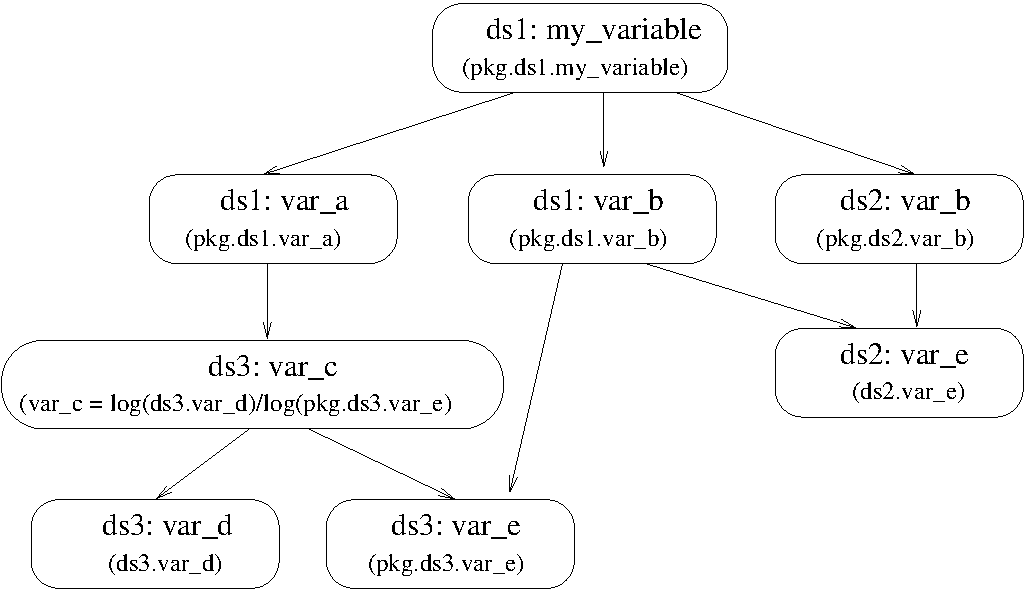
\includegraphics[scale=0.6]{images/variabletreeinitial.pdf}
%end{latexonly}
\caption{\label{fig:opus-core-variable-tree}\small Example of a variable
  dependencies tree. The arrows indicate the dependency direction: 
  $a \longrightarrow b$ means '$a$ is dependent on $b$'.}
\htmlonly{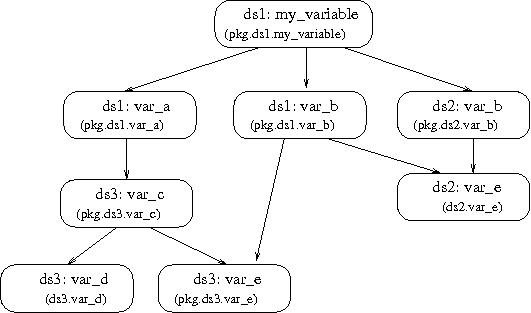
\includegraphics[scale=0.9]{images/variabletreeinitial.jpg}}
\end{center}
\end{figure}

As an example, consider Figure~\ref{fig:opus-core-variable-tree}. There are 8
variables/attributes,  belonging to 3 datasets, \verb|ds1|, \verb|ds2|, and
\verb|ds3|.  The arrows show the dependency hierarchy between variables. The
hierarchy is defined in the method \method{dependencies()} of each variable
by listing all direct 'children' variables as expressions, fully-qualified names or dataset-qualified names (in
this example the names in the parentheses in the figure). Note that two
attributes here are primary, namely ``ds3.var_d'' and ``ds2.var_e'', and
thus are defined in their dataset-qualified name (there is no variable
implementation for those attributes). For example, the \method{dependencies()} method of the root variable 
``pkg.ds1.my_variable'' returns a list of three elements: \verb|['pkg.ds1.var_a', 'pkg.ds1.var_b', 'pkg.ds2.var_b']|, 
and \method{dependencies()} of the variable ``pkg.ds1.var_a'' returns a list with one expression:
\verb|['var_c = log(ds3.var_d)/log(pkg.ds3.var_e)']|. As described in Section~\ref{sec:implementation-of-expressions}, 
expressions do not have user-defined implementations (they are created on the fly). Therefore there is 
no need to define dependencies for the variable ``ds3.var_c'', Opus determines them automaticaly. 

Now suppose we have a system of several models, three of which are invoking
the computation of ``my_variable'' of dataset \verb|ds1|. Suppose also that
initially we have created the three datasets and loaded the two primary
attributes.  Opus assigns to each newly created attribute a version number 0 in
its attribute box.  This situation is shown in the left upper corner of
Figure~\ref{fig:opus-core-variable-tree-1}. Box number 1 shows that there are only
two attributes in the system, both with version number 0.

\begin{figure}
\begin{center}
%begin{latexonly}
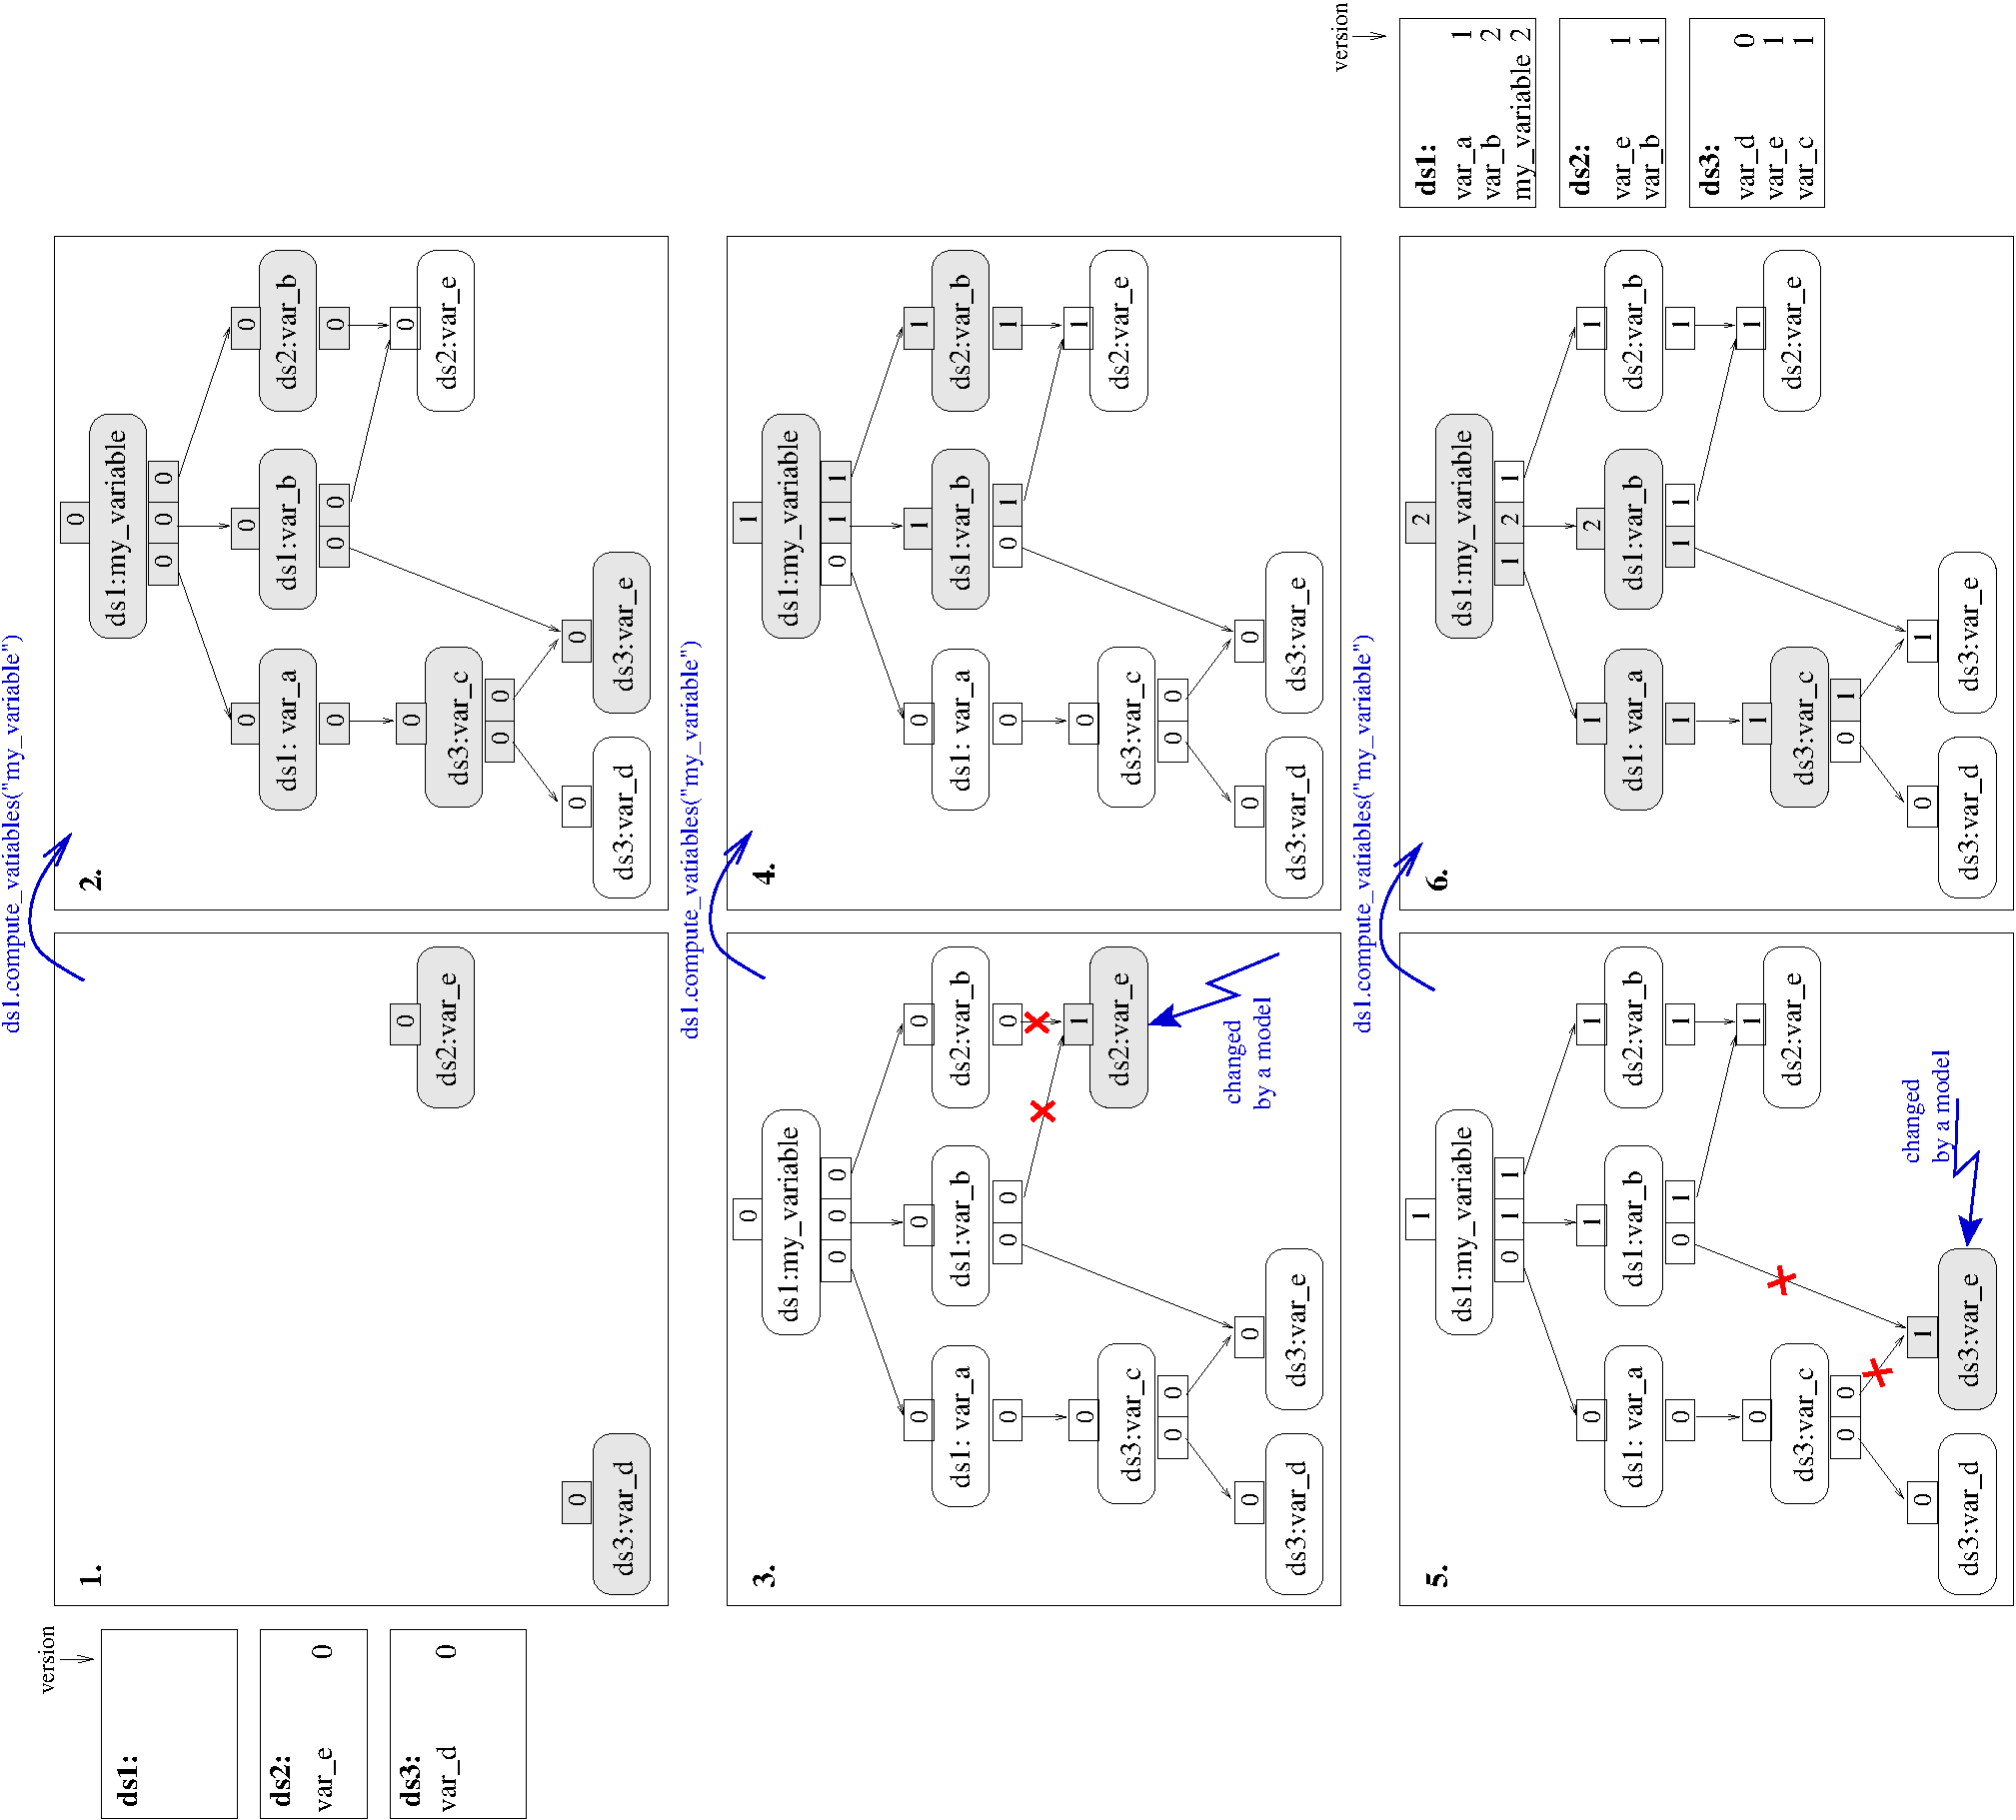
\includegraphics[scale=0.55, angle=-90]{images/variabletree1.pdf}
%end{latexonly}
\caption{\label{fig:opus-core-variable-tree-1}\small Scenario of computing and
  recomputing variables.}
\htmlonly{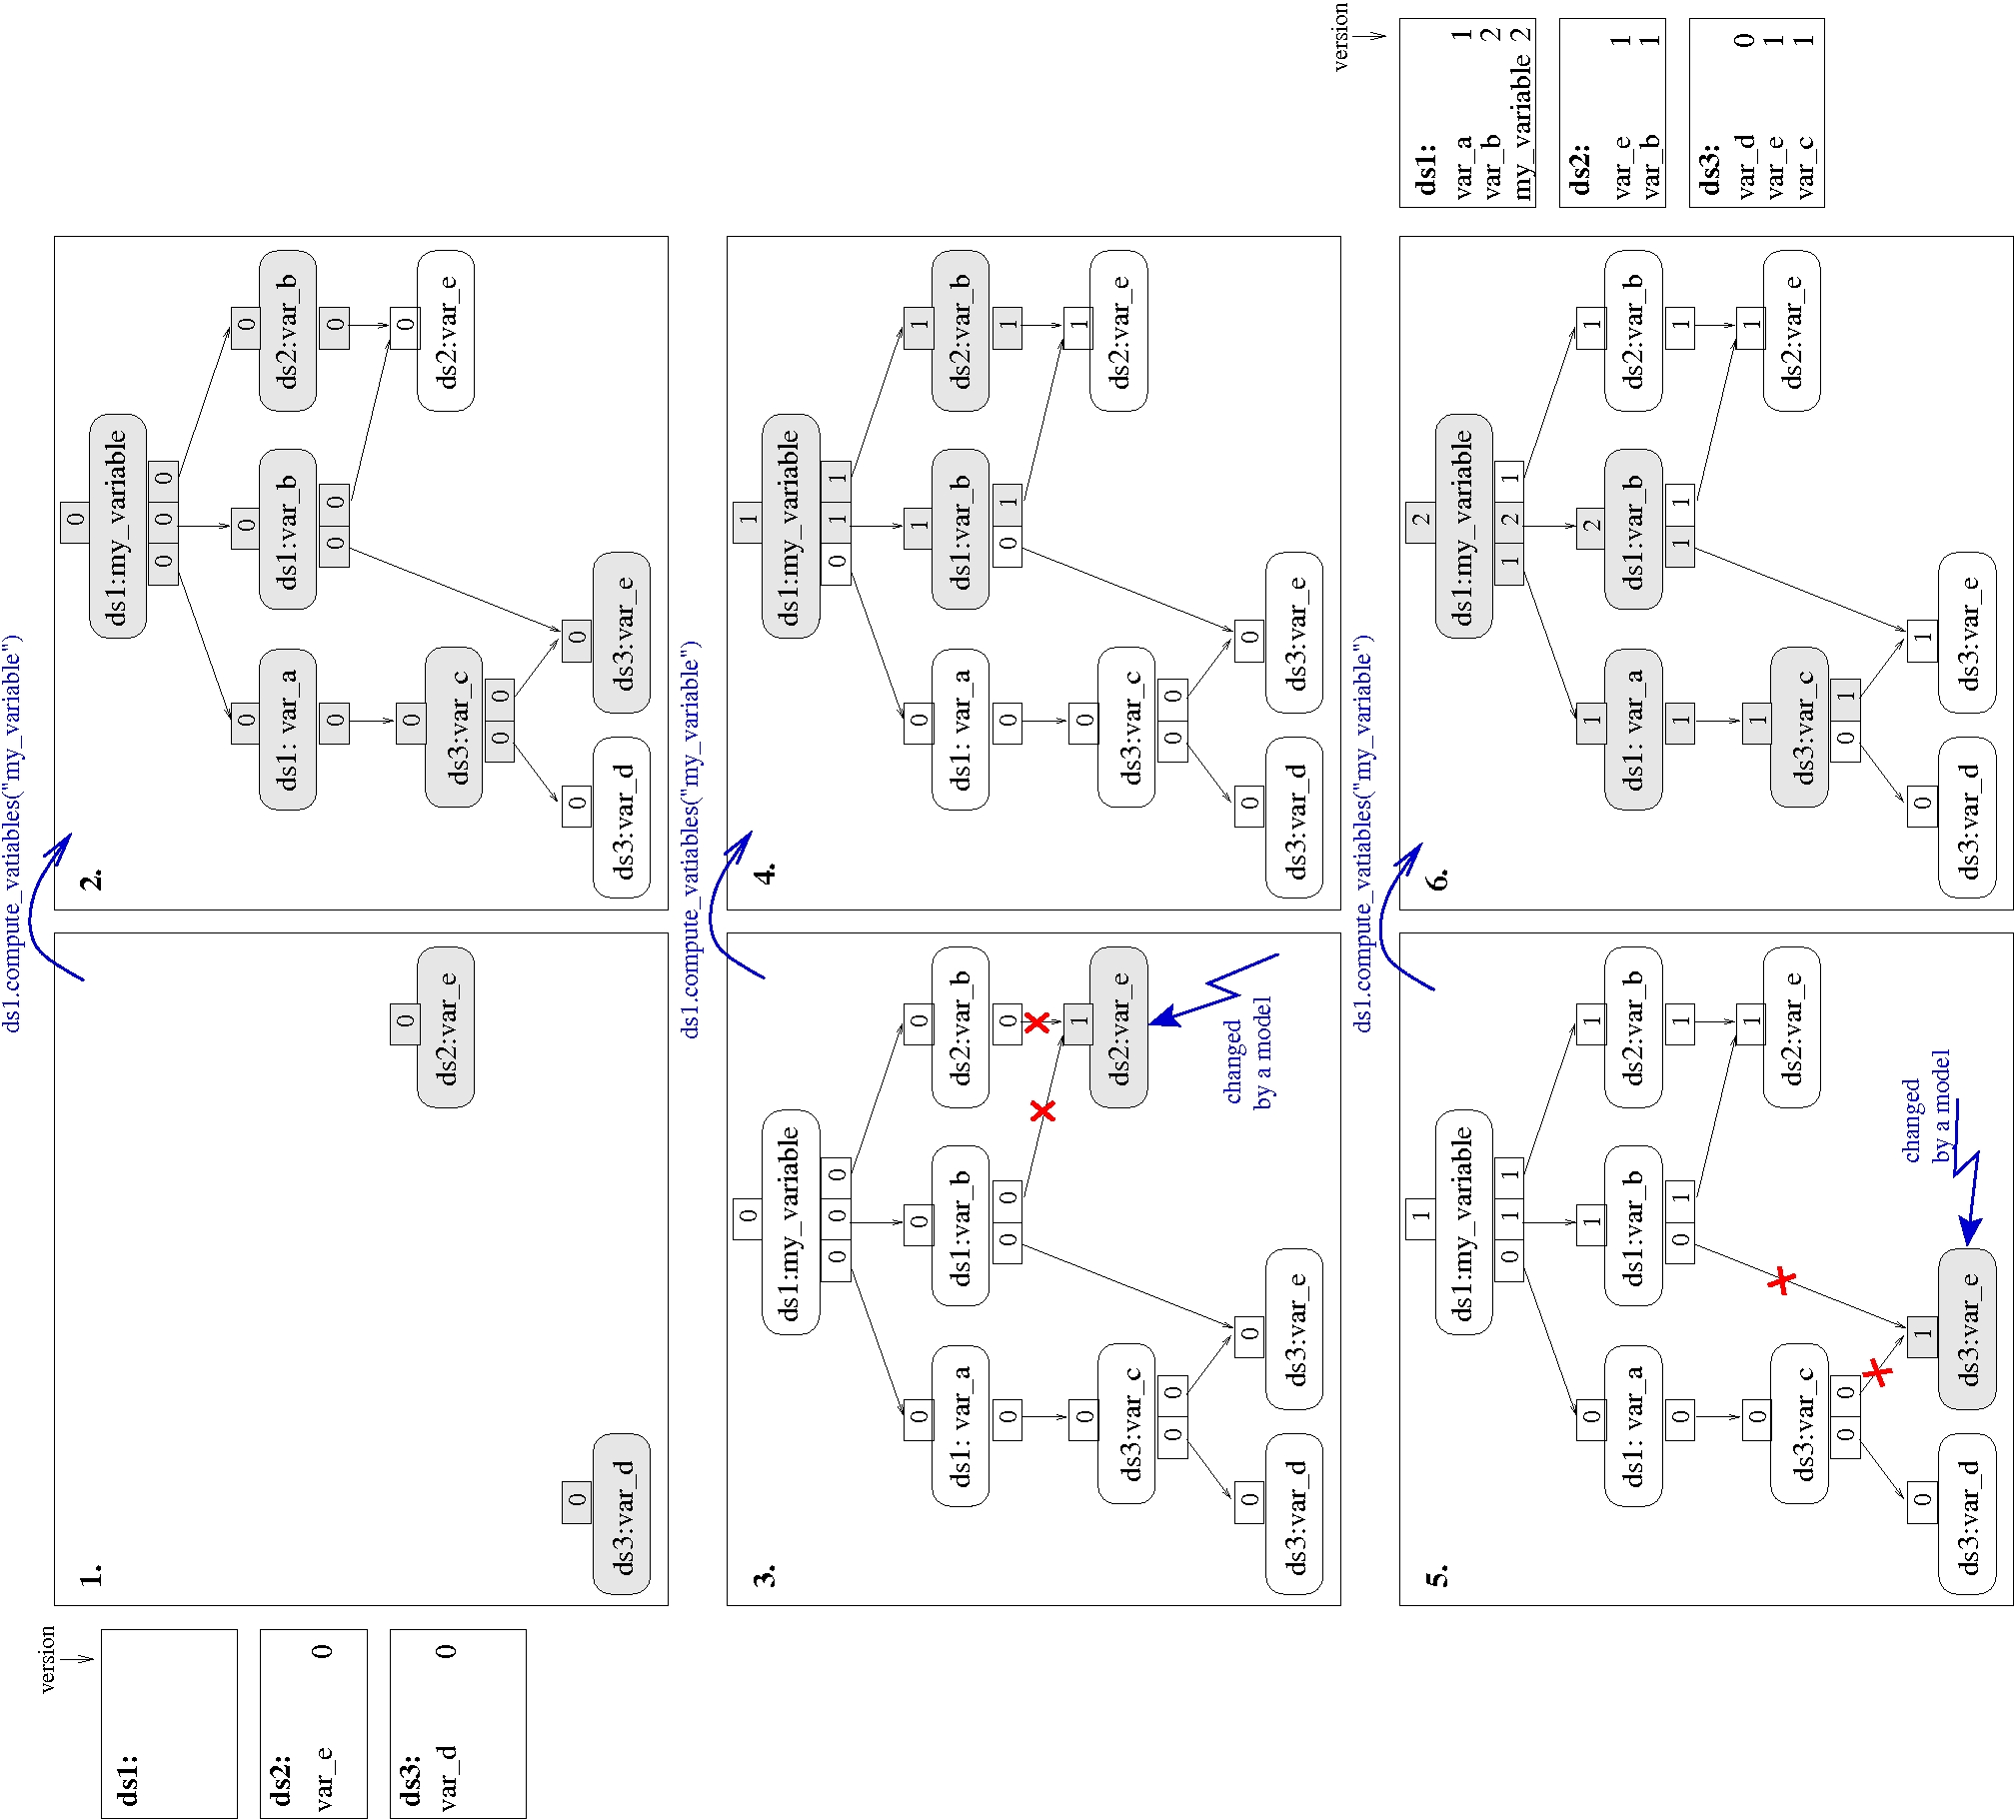
\includegraphics[scale=0.55, angle=-90]{images/variabletree1.jpg}}
\end{center}
\end{figure}

Box 2 shows a situation when the first model invokes the computation of
``my_variable'' \footnote{Because of the dependencies on variables of other
  datasets, the correct call is\\
  \code{ds1.compute_variables(["pkg.ds1.my_variable"], dataset_pool=pool)} where \code{pool}
  is constructed as described in Section~\ref{sec:core-dataset-pool} and contains datasets ``ds2'' and ``ds3''.
  We simplify the notation here for
  a better readability.}. The system works through the defined dependencies and
computes all variables needed to compute ``my_variable''. In this process,
again, each newly computed variable gets the version number 0 (illustrated by
the small boxes above each variable), stored in the attribute box of each
variable. Additionally, each \class{Variable} instance keeps the version
number for each dependent variable, on which this variable was computed. In
the figure, this is illustrated by the small boxes bellow each variable.
Note that all elements in Figure~\ref{fig:opus-core-variable-tree-1} that are
created or change their values are shaded.

The box number 3 shows a situation in which another model changes values of
variable ``var_e'' of the dataset \verb|ds2| which causes an increment of the
version number. Therefore, when the next model invokes
\method{compute_variables("my_variable")}, Opus determines that there is a
mismatch between versions of ``ds.var_e'' on which variables ``ds1.var_b'' and
``ds2.var_b'' were computed and its current version (the mismatch is visualized by red crosses). Then all
variables above ``ds.var_e'' are recomputed, their version numbers
incremented, and the version numbers in the dependencies lists are updated
(box 4).

A similar situation arises when another model changes the variable
``ds3.var_e'' (box 5). The next call of
\method{compute_variables("my_variable")} causes a recomputing of 4
variables (box 6) In the right lower corner of
Figure~\ref{fig:opus-core-variable-tree-1}, the state of the three datasets is
shown at the end of the run of our example models.

Note that the dependencies tree is constructed using the
\method{dependencies()} method of \class{Variable}. Therefore a missing item
in this method translates to a missing branch of the tree and thus failing to
determine a need for recomputing.


\subsection{Expression Language Implementation}
\label{sec:implementation-of-expressions}
\index{expressions!implementation}

Opus expressions are written in a domain-specific programming language called Tekoa
(Chapter~\ref{chapter:expressions}).  Each newly-encountered expression is compiled into
an automatically generated subclass of \class{Variable}, with similar functionality
to that described above.  This section describes how this compilation is done.
For the most part, the implementation shouldn't be relevant
to the Opus user.  But for the curious, for programmers who want to modify or extend
the system, or (heaven forfend) in case something goes wrong, here is a
description of the implementation.  The code to implement expressions is in
\package{opus_core.variables}.  

Regarding Tekoa extensions, one straightforward extension is to add additional 
functions to the language.  The currently available unary functions are 
listed in Section \ref{sec:functions-for-opus-expressions}.  These all operate 
on numpy arrays.  Additional functions in the domain-specific
language can be supported by adding additional definitions to 
\package{opus_core.variables.functions}.  (If you believe this extension would
be of general interest, please coordinate with the Opus/UrbaSim implementors
so that it can find its way into the code base.)

When a new expression is encountered, the system automatically compiles a
new subclass of \class{Variable} that implements the computation defined by
that expression.  If the expression is a simple attribute or
fully-qualified variable, evaluating the expression reduces to getting the
value of the attribute or computing the value of the existing
variable. Otherwise, the expression system generates and compiles a new
variable to implement an expression. It keeps a cache of expressions that
have already been processed, so that autogenerated variables can be reused
when possible. These autogenerated variables have names like
\class{autogenvar034}. They are compiled and live just in the current
process --- they aren't stored on disk, so that the user never needs to see
them, and so that different processes running on the same machine don't
interfere with each other.

Since expressions use standard Python syntax, they can be parsed using the
standard Python parser module, rather than needing to write one. The parse
tree for the expression is analyzed and the dependencies extracted to
generate the dependencies method --- the user doesn't need to declare the
dependencies for an expression. The \method{compute()} method for the
autogenerated variable includes the user's expression directly as part of
the method.  To enable this to work correctly, the method includes
statements to set up the local environment in the method so that all of the
names are properly bound.  Here is an example.  Suppose the input
expression is \verb|ln_bounded(urbansim.gridcell.population)|.  Then the
automatically generated class will be:
\begin{verbatim}
class autogenvar034(Variable):
    def dependencies(self):
        return ['urbansim.gridcell.population']
    def name(self):
        return 'ln_bounded(urbansim.gridcell.population)'
    def compute(self, dataset_pool):
        urbansim = DummyName()
        urbansim.gridcell = DummyDataset(self, 'gridcell', dataset_pool)
        urbansim.gridcell.population = \
            self.get_dataset().get_attribute('population')
        return ln_bounded(urbansim.gridcell.population)
\end{verbatim}

The name of the class is generated (there is a class variable
autogen_number in the class \class{AutogenVariableFactory} that starts at 0
and gets incremented each time it's used in a new name).

The dependencies method is constructed by parsing the expression and
finding all of the other variables that it references, and putting those
into the returned list.

The compute method ends with a return statement that just returns
\code{expr}.  To make this work, we need to provide local bindings for
e.g. \code{urbansim.gridcell.population}.  We bind a local variable (named
\code{urbansim} in the example) to an instance of \class{DummyName}, whose
sole purpose in life is to have an attribute gridcell (and maybe other
attributes if there are multiple dependencies).  Then
\code{urbansim.gridcell} is bound to an instance of \class{DummyDataset},
which is used in place of a real dataset in the autogenerated code.  We
then add a population attribute to \code{urbansim.gridcell}, bound to the
value of the appropriate dataset attribute.  (We use the dummy dataset
rather than adding attributes to the real dataset, which might interfere
with other attributes or not be garbage-collected as soon as they might
otherwise be.)  For the get_attribute call to get the value of the
population attribute, we use the short version of the name -- its value
should already have been computed by virtue of being listed in the
\method{dependencies()} method.

If the expression includes an alias, for example
\verb|pop = ln_bounded(urbansim.gridcell.population)|, then the code is all
the same as above, except that the final return statement is replaced with
\begin{verbatim}
            pop = ln_bounded(urbansim.gridcell.population)
            return pop
\end{verbatim}

The \method{aggregate}, \method{disaggregate}, and \method{number_of_agents}
methods are defined on \class{DummyDataset}, so that they can be used in
expressions.

\section{Models} 
\index{models!opus_core models}
\label{sec:opus-core-models}

The \package{opus_core} package offers a few simple models that can serve as parent classes
for user specific models or can be used directly. Their hierarchy is shown in
Figure~\ref{fig:opus-core-model}. \class{Model} and \class{ChunkModel} are abstract
classes, each of the remaining models implements a specific 
functionality. The classes are described in detail in the next sections.

\begin{figure}
\begin{center}
%begin{latexonly}
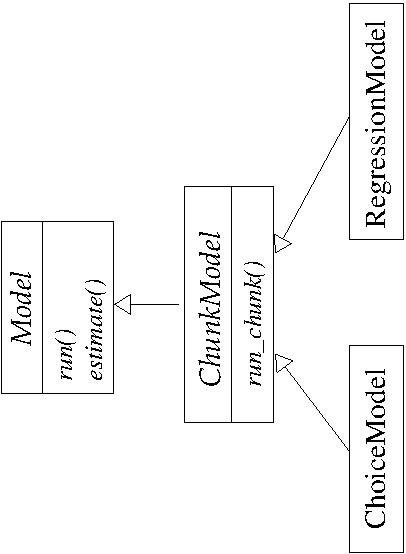
\includegraphics[scale=0.8]{images/coremodelswithmethods.pdf}
%end{latexonly}
\caption{\label{fig:opus-core-model}\small Models in \package{opus_core}. Arrows indicate the inheritance hierarchy:
$a \rightarrow b$ means $a$ inherits from $b$.}
\htmlonly{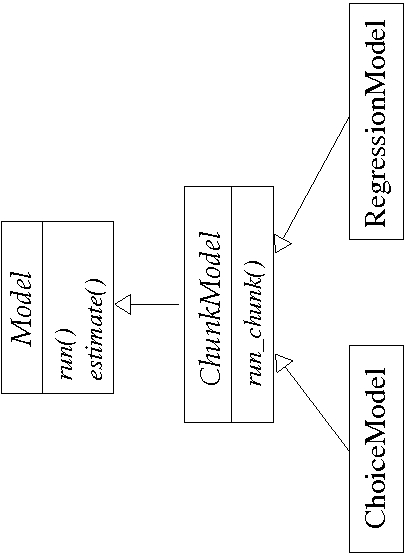
\includegraphics[scale=0.8]{images/coremodelswithmethods.jpg}}
\end{center}
\end{figure}

\subsection{Model Class}
\index{Model@\class{Model} class}
\class{Model} is the base class for implementing Opus models. It provides an
automatic logger which prints out information about the model start, end and
processing time.  Model supports two methods: an obligatory method
\method{run()} and an optional method \method{estimate()}. Each child of
\class{Model} can define a class attribute \verb|model_name| that is used as
an identification of the specific model in the logger output. Any arguments
can be passed into the \method{run()} and \method{estimate()} methods and
those can return any values.

\subsection{ChunkModel Class}
\label{sec:chunk-model} \index{ChunkModel@\class{ChunkModel} class}
\index{Memory management!Using multiple chunks per model}

This class enables running models (i.e. processing the \method{run()} method) in
several chunks, for example if a run of the whole model would require too much
memory. The class does not have any effect on an \method{estimate()} method.

\subsubsection{The Run Method}
{\it Input}:
\begin{description}
\item[chunk_specification] - a dictionary specifying how to determine the number
  of chunks to run the model in. It must contain either the key 'records_per_chunk'
  or the key 'nchunks'. The method passes it to the constructor of \class{ChunkSpecification} 
  (see Section~\ref{sec:resources}). None translates to 1 chunk. 
\item[dataset] - an object of class \class{Dataset} along whose elements the
  model will be chunked.
\item[dataset_index] - an index of elements within \verb|dataset| that are to
  be chunked. Default is None which means that all elements of \verb|dataset| are considered.
\item[result_array_type] - a type of the resulting array. It can be any numerical type of numpy array.
        The default value is \verb|float32|.
\item[...] - optional additional arguments that are passed to the method
  \method{run_chunk()}. They are expected to be keyword arguments.
\end{description}


{\it Algorithm}:~\\[1mm]
%
For each chunk (determined by the \verb|chunk_specification|) the model calls
the method \method{run_chunk()} and passes as arguments the corresponding portion
of \verb|dataset_index|, the whole \verb|dataset| and all additional
arguments. By default the order of elements in \verb|dataset_index| is
preserved. This can be changed by redefining the method
\method{get_agents_order()} (see below). 

{\it Output}:~\\[1mm]
%
The class returns an array of the same size as \verb|dataset_index| and of type \verb|result_array_type| 
(passed to the method as input).
Values of this array are return values of the (possibly) multiple calls of the method \verb|run_chunk()|.
The $i$-th value in this array is a result for the \verb|dataset_index|[$i$]-th element of \verb|dataset|.

\subsubsection{Implementing a Child Class}
%
All models that are derived from the ChunkModel class must have the method \method{run_chunk()} implemented. 
It has two non-keyword arguments: an integer array and an object of class \class{Dataset}. The first argument 
is an index of elements within the second argument. The method can have additional keyword arguments.  
The method is expected to return an array of the same size as the size of the first argument (i.e. the chunk size).
The $i$-th value of the result is expected to be associated with the dataset element indexed by index[$i$].

Optionally, the method  \method{get_agents_order()} can be implemented in the child class. It determines the order in which 
dataset elements are passed into chunks. This method takes a dataset as an argument which is an
object of class \class{DatasetSubset}\index{DatasetSubset@\class{DatasetSubset} class} containing only those elements of the
original \verb|dataset| that are defined by \verb|dataset_index|.  It returns
an index of elements within the given subset determining the order in which the
elements should be processed. For example, if this method returns a randomized
index, the elements passed into \method{run_chunk()} will be processed in
randomized order.

An example of a user-defined \class{ChunkModel} is in Section~\ref{sec:tut-creating-new-model}.

\subsection{ChoiceModel Class}
\label{sec:choice-model}
\index{ChoiceModel@\class{ChoiceModel} class}
\index{models!opus_core models!choice model}
%
This class implements a functionality of a discrete choice model, an approach
widely used in land use and transportation modeling. In principal, a set of
agents make choices from a finite set of possibilities (alternatives). The
choice selection is based on probabilities derived from utilities. These are
computed on the basis of given variables and coefficients. The model allows
the coefficients to be also estimated within this framework. See also Section~\ref{sec:components-choice-model}.

As there are many different aspects to consider in specifying a discrete
choice model, the software has been designed in a modular way to accommodate
substantial flexibility in configuring these models. Each component included
in the model is passed as character string that determines the module$=$class
name (as a fully qualified name) in which the component is implemented.

\subsubsection{Initialization}
%
The class is initialized by passing the following arguments:
\begin{description}
\item[choice_set] - A list, array or dataset that represents the finite set of
  possible choices. It should have numeric values larger than zero.
\item[utilities] - A fully qualified name of the module for computing utilities
  (see Section~\ref{sec:utilities}). Default value is
  \verb|'opus_core.linear_utilities'|.
\item[probabilities] - A fully qualified name of the module for computing
  probabilities (see Section~\ref{sec:probabilities}). Default value is
  \verb|'opus_core.mnl_probabilities'|.
\item[choices] - A fully qualified name of the module for determining
  final choices (see Section~\ref{sec:choices}). Default value is
  \verb|'opus_core.random_choices'|.
\item[submodel_string] - If model contains submodels, this character string
  specifies what agent' attribute determines those submodels. Default is None, i.e. no submodels.
\item[choice_attribute_name] - Name of the attribute that identifies the
  choices. This argument is only relevant if \verb|choice_set| is not an
  instance of \class{Dataset}. Otherwise the choices are identified by the
  unique identifier of the \verb|choice_set|. Default value is
  \verb|'choice_id'|
\item[interaction_pkg] - This argument is only relevant if there is an
  implementation of an interaction dataset that corresponds to interaction
  between agents and choices. It is the name of the Opus package where the implementation lives.
  Default value is \verb|'opus_core'|.
\item[run_config] - A collection of additional arguments that control a
  simulation run. It should be of class \class{Resources}. Default is None.
\item[estimate_config] - A collection of additional arguments that control an
  estimation run. It should be of class \class{Resources}. Default is None.
\item[dataset_pool] - A pool of datasets needed for computation of variables. Default is None.
\end{description}
The initialization method creates a class attribute \verb|upc_sequence|, using
the passed arguments \verb|utilities|, \verb|probabilities| and
\verb|choices|. It is an object of class \class{upc_sequence} (see
Section~\ref{sec:upc-sequence}). A class attribute \verb|choice_set| is an
object of \class{Dataset}. If the argument \verb|choice_set| is a list or
array, a \class{Dataset} is created using the values of the argument as the
unique identifier. The name of this unique identifier is the value of \verb|choice_attribute_name|.

\subsubsection{The Run Method}
%
The \method{run()} method runs the simulation on basis of a given specification
and coefficients\index{coefficients}.

{\it Input}:
\begin{description}
\item[specification] - an instance of class \class{EquationSpecification}
  specifying variables to be used in the simulation (see Section~\ref{sec:specification}).
\item[coefficients] - an instance of class \class{Coefficients} that contains
  values of coefficients to be used in the simulation (see Section~\ref{sec:coefficients}).
\item[agent_set] - an instance of class \class{Dataset} representing the whole
  set of agents to be used for the variable computation.
\item[agents_index] - an index within the \verb|agent_set| determining which
  agents enter the choice process. If it is not given (default), all agents are
  considered.
\item[chunk_specification] - a dictionary specifying how to determine the number
  of chunks to run the model in. It is  passed to the \method{run} method of \class{ChunkModel}
   (see Section~\ref{sec:chunk-model}). 
  Default is None, which is equivalent to 1 chunk.
\item[data_objects] - a dictionary containing additional datasets 
  needed for computing variables. This argument is obsolete -- the datasets should be 
  included in the \verb|dataset_pool| argument of the constructor.
\item[run_config] - additional \class{Resources} for controlling the
  simulation run.
\end{description}


{\it Algorithm}:~\\[1mm]
The algorithm is implemented in the method \verb|run_chunk()| called from the
parent class \verb|ChunkModel| for each chunk. It overwrites the
\class{ChunkModel} method \verb|get_agents_order()| in a way that it returns a
permutation of the agents indices. Thus, the agents make their choices in a
random order.

The method creates an interaction set between the agent set and the choice
set. It computes all variables given in the specification. Variables that are
specific to one of the datasets are computed on all elements of that dataset, 
interaction variables are computed only on elements entering the choice
process. The method then creates the corresponding data matrix using
\verb|agents_index| for selecting the appropriate data values. It runs one
simulation per submodel (for submodels specified in the specification) by
calling the \verb|run()| method of the \verb|upc_sequence| attribute
(see~\ref{sec:upc-sequence}) and passing the data matrix and the coefficients
for the corresponding submodel.

If \verb|run_config| contains the entry 'demand_string' having a character string value, 
an aggregated demand for each choice is computed and stored as an additional attribute (of that name)
of the choice dataset.

{\it Output}:~\\[1mm]
The method returns an array of size \verb|agents_index|, representing the
choices that agents (elements of \verb|agent_set| determined by
\verb|agents_index|) made. Agents whose choice is less equal zero  were
not included in the choice process, for example because they do not belong to
any submodels given in the specification.

\subsubsection{The Estimate Method}
%
The \method{estimate()} method runs an estimation of coefficients on basis of
a given specification.

{\it Input}:
\begin{description}
\item[specification] - an instance of class \class{EquationSpecification}
  specifying variables to be used in the estimation (see Section~\ref{sec:specification}).
\item[agent_set] - a \class{Dataset} representing the whole set of agents
  to be used for the variable computation.
\item[agents_index] - an index within the \verb|agent_set| determining which
  agents will be used for the estimation. If it is not given (default), all agents are
  considered.
\item[procedure] - a character string giving the fully qualified name of the
  estimation procedure (see Section~\ref{sec:estimation-procedure}). This argument can be also passed via
  \verb|estimate_config| as an entry \verb|'estimation'|. The default value is None.
\item[data_objects] - a dictionary containing additional datasets 
  needed for computing variables. This argument is obsolete -- the datasets should be 
  included in the \verb|dataset_pool| argument of the constructor.
\item[estimate_config] - additional \class{Resources} for controlling the
  estimation run.
\end{description}

{\it Algorithm}:~\\[1mm]
In addition to \verb|agents_index|, the number of agents entering the
estimation can be controlled by an entry \verb|'estimation_size_agents'| in
\verb|estimate_config| which should have a value between $0$ and $1$. It gives
the portion of \verb|agents_index| (or \verb|agent_set| if \verb|agents_index|
is not given) that will be used in the estimation. The indices are then
randomly sampled. The \verb|agent_set| should contain an attribute of the same
name as the unique identifier of the class attribute \verb|choice_set|. Its
values determine the current choices of the agents.

As in the \method{run()} method, an interaction set is created and the
variables given in the specification are computed. Then for each submodel the
corresponding data matrix is built and the \verb|run()| method of the class
given by the argument \verb|procedure| (or alternatively by an entry
``estimation'' in \verb|estimate_config|) is called, passing the data array,
the class attribute \verb|upc_sequence| and \verb|estimate_config| (after
adding entries needed for the estimation) as arguments (see
Section~\ref{sec:estimation-procedure} for more details).  From the returned
dictionary, items ``estimators'', ``standard_errors'', ``other_measures'' and
``other_info'' are extracted. After results from all submodels are collected,
a \class{Coefficient} object is created using those extracted values (see Section~\ref{sec:specification}).

{\it Output}:~\\[1mm]
The method returns a tuple of the created \class{Coefficient} object and a
dictionary with one entry for each submodel. 
Each entry is a dictionary returned by estimation procedure for that submodel.

\subsection{RegressionModel Class}
\index{RegressionModel@\class{RegressionModel} class}
\index{models!opus_core models!regression model}
%
\label{sec:regression-model}
The \class{RegressionModel} class implements a model based on a regression
procedure. In summary, there is a set of observations, whose attributes or/and
variables are used to predict a certain outcome, using some coefficients.
Those can be also estimated within this framework. See also Section~\ref{sec:components-regression-model}.

As in the case of \class{ChoiceModel}, the regression model can be composed by
plug-in modules.

\subsubsection{Initialization}
The class is initialized by passing the following arguments:
\begin{description}
\item[regression_procedure] - a fully qualified name of the module/class in
  which the regression is implemented (see Section~\ref{sec:regression}).
  The default value is 'opus_core.linear_regression'.
\item[submodel_string] - If model contains submodels, this character string
  specifies what attribute of the observation set determines those submodels. Default is None.
\item[run_config] - A collection of additional arguments that control a
  simulation run. It should be a dictionary or an instance of class \class{Resources}. Default is None.
\item[estimate_config] - A collection of additional arguments that control an
  estimation run. It should be a dictionary or an instance of class \class{Resources}. Default is None.
\item[dataset_pool] - A pool of datasets needed for computation of variables. Default is None.
\end{description}
From the argument \verb|regression_procedure| the initialization method
creates a class attribute \verb|regression|, using
\class{RegressionModelFactory} (see Section~\ref{sec:model-components}).
The remaining arguments are set as class properties.

\subsubsection{The Run Method}
%
The \method{run()} method runs the simulation on basis of a given
specification and coefficients.

{\it Input}:
\begin{description}
\item[specification] - an instance of class \class{EquationSpecification}
  specifying variables to be used in the simulation.
\item[coefficients] - an instance of class \class{Coefficients} that contains
  values of coefficients to be used in the simulation.
\item[dataset] - a \class{Dataset} representing the whole set of observations.
\item[index] - an index within \verb|dataset| determining for which
  observations the prediction is to be made. If it is not given, the whole
  \verb|dataset| is considered.
\item[chunk_specification] - a dictionary specifying how to determine the number
  of chunks to run the model in. It is  passed to the \method{run} method of \class{ChunkModel}
   (see Section~\ref{sec:chunk-model}).
\item[data_objects] - a dictionary containing additional datasets 
  needed for computing variables. This argument is obsolete -- the datasets should be 
  included in the \verb|dataset_pool| argument of the constructor.
\item[run_config] - additional \class{Resources} (or dictionary) for controlling the simulation
  run.
\item[initial_values] - an array of initial values of the results. It is of the same size as 
  \verb|dataset|. Elements that are handled by the model (determined by \verb|index| and specification)
  will be overwritten by the results. By default, the array is set to zeros.
\item[procedure] - a fully qualified name of the module/class in
  which the regression is implemented (see Section~\ref{sec:regression}). 
  If it is None (default), the value of \verb|regression_procedure| from the constructor is taken. 
  This argument overwrites the class attribute \verb|regression|.

\end{description}

{\it Algorithm}:~\\[1mm]
The algorithm is implemented in the method \verb|run_chunk()| called from the
parent class \class{ChunkModel} for each chunk. It invokes a computation of
all variables given in the specification. Then for each submodel it creates a
data matrix for values corresponding to \verb|index| and invokes the
\verb|run()| method of the object stored in the class attribute
\verb|regression| (see Section~\ref{sec:regression}).

{\it Output}:~\\[1mm]
The method returns an array of the same size as \verb|index|, determining the
outcome of the regression for each observation included in \verb|index|.

\subsubsection{The Estimate Method}
The \method{estimate()} method runs an estimation of coefficients on basis of
a given specification.

{\it Input}:
\begin{description}
\item[specification] - an instance of class \class{EquationSpecification}
  specifying variables to be used in the estimation.
\item[dataset] - a \class{Dataset} representing the whole set of observations.
\item[outcome_attribute] - a character string determining the dependent
  variable (a fully qualified name).
\item[index] - an index within the \verb|dataset| determining which
  observations will be used for the estimation. If it is not given, the whole
  \verb|dataset| is considered.
\item[procedure] - a character string giving the fully qualified name of the
  estimation procedure (see Section~\ref{sec:estimation-procedure}). This argument can be also passed via
  \verb|estimate_config| as an entry \verb|'estimation'|. The default value is None.
\item[data_objects] - a dictionary containing additional datasets 
  needed for computing variables. This argument is obsolete -- the datasets should be 
  included in the \verb|dataset_pool| argument of the constructor.
\item[estimate_config] - additional \class{Resources} (or dictionary) for controlling the
  estimation run.
\end{description}

{\it Algorithm}:~\\[1mm]
In addition to \verb|index|, the number of dataset members entering the
estimation can be controlled by an entry \verb|'estimation_size_agents'| in
\verb|estimate_config| which should have a value between $0$ and $1$. It gives
the portion of \verb|index| that will be used in the estimation. If it is less than 1, 
the indices are randomly sampled.

The method invokes computation of variables given in the specification as well
as of the outcome attribute. For each submodel, it creates the corresponding
data matrix and invokes the \verb|run()| method of the module given by the
argument \verb|procedure|, passing data, the class attribute \verb|regression|
and \verb|estimate_config| (after adding entries needed for the estimation) as
arguments (see Section~\ref{sec:estimation-procedure} for more details). From
the returned dictionary, items ``estimators'', ``standard_errors'',
``other_measures'' and ``other_info'' are extracted.  After results from all
submodels are collected, a \class{Coefficient} object is created using those
extracted values.

{\it Output}:~\\[1mm]
The method returns a tuple of the created \class{Coefficient} object and a
dictionary with one entry for each submodel. 
Each entry is a dictionary returned by estimation procedure for that submodel.

\subsubsection{Child Class RegressionModelWithInitialResiduals}
\index{RegressionModelWithInitialResiduals@\class{RegressionModelWithInitialResiduals} class}
\label{page:regression-model-with-initial-residuals}
%
This class impacts only the method \method{run()} (it doesn't change the behaviour of the \method{estimate()} method).
It computes initial errors of the observations to the predictions (residuals)
if run for the first time. The error values are added to \verb|dataset| as a primary attribute 
(with the same name as the outcome attribute adding the prefix '_init_error_').
Then in any run, the error is added to the outcome. Thus, in order to compute the residuals,
the outcome attribute must be a known attribute of \verb|dataset| prior to running the model.
Note that running this model on the same set of observations which were used for the estimation,
should result in the same outcome as the original values of the outcome attribute.

In addition to all parents arguments, this class requires the argument \verb|outcome_attribute|
to be passed into the constructor. The following entries of the \verb|run_config| dictionary are accepted:
\begin{itemize}
\item 'exclude_missing_values_from_initial_error' - default is False.
\item 'outcome_attribute_missing_value' - if the above entry is True, this value determines a missing value. Default is 0.
\item 'exclude_outliers_from_initial_error' - default is False.
\item 'outlier_is_less_than' - lower bound for excluding outliers from computing residuals.
\item 'outlier_is_greater_than' - upper bound for excluding outliers from computing residuals.
\end{itemize}

\subsection{SimpleModel Class}
\label{sec:api-simple-model}
\index{SimpleModel@\class{SimpleModel} class}
\index{models!opus_core models!simple model}
%
This model is an alternative way of computing a variable on a dataset, except that the resulting attribute 
becomes a primary attribute (see also Section~\ref{sec:components-simple-model}).

The \method{run()} method takes the following arguments:
\begin{description}
\item[dataset] an object of class \class{Dataset} for which the computation is done.
\item[expression] - any variable or expression that can be computed on \verb|dataset|.
\item[outcome_attribute] - name of the outcome attribute. If it is None (default), alias
of the \verb|expression| is taken.
\item[dataset_pool] - pool of datasets passed into the computation. Default is None.
\end{description}

The \method{run()} method computes the given expression on the given dataset. If the \verb|outcome_attribute| already exists
on the dataset, it is deleted. Results from the computation are assigned to \verb|outcome_attribute| and 
the attribute is marked as primary. Values of this attribute are returned.

\subsection{AllocationModel Class}
\label{sec:api-allocation-model}
\index{AllocationModel@\class{AllocationModel} class}
\index{models!opus_core models!allocation model}
%
The AllocationModel allocates given quantity for a dataset according to weights while meeting capacity restrictions 
(see Section~\ref{sec:components-allocation-model}). 

The \method{run()} method takes the following arguments:
\begin{description}
\item[dataset] - an object of class \class{Dataset} for which the allocation is done.
\item[outcome_attribute] - name of the resulting attribute.
\item[weight_attribute] - an attribute/variable/expression of \verb|dataset| which determines weights for the allocation.
\item[control_totals] - an object of class \class{Dataset} holding data with the total amount of quantity to be allocated.
\item[current_year] - integer value used for filtering out control totals for the current year. 
\item[control_total_attribute] - name of the attribute in \verb|control_totals| that specifies the total amount to be allocated.
  If it is not given, the value of \verb|outcome_attribute| is taken.
\item[year_attribute] - name of the attribute in \verb|control_totals| on which the filtering 
of the current year is done. Default is 'year'.
\item[capacity_attribute] - name of the attribute/variable/expression in \verb|dataset| specifying capacity for each member. 
  Default is None which means there are no capacity restrictions. 
\item[add_quantity] - if True and the \verb|outcome_attribute| exists in \verb|dataset|, 
  the resulting values are added to the current values of 
    \verb|outcome_attribute|. Default is False.
\item[dataset_pool] - pool of datasets used in the computation. Default is None.
\end{description}

In addition to the \verb|year_attribute| and \verb|control_total_attribute|, the \verb|control_totals| dataset 
can contain other attributes that must be known to the \verb|dataset| (such as a geography), here called 'common' attributes.
For each row of the \verb|control_totals| that matches the current year,
the total amount is distributed among members of \verb|dataset| that have the same values of all common attributes as the row.
The distribution is done using the given weights. 
If the \verb|capacity_attribute| is given, the algorithm removes any allocations that exceeds the capacity and 
re-distributes it among remaining members. The resulting values are appended 
to \verb|dataset| as 
\verb|outcome_attribute| which is marked as primary.
If \verb|add_quantity| is True, the resulting values are added to the current values of 
        \verb|outcome_attribute| if it exists. 
The \verb|outcome_attribute| is then flushed to cache and the values are returned.
        
        
\subsection{JoinAttributeModificationModel Class}
\label{sec:api-jam-model}
\index{JoinAttributeModificationModel@\class{JoinAttributeModificationModel} class}
%
The model modifies an attribute of a dataset for members that are determined by given ids of a second dataset.
The \method{run()} method takes the following arguments:
\begin{description}
\item[dataset] - an object of class \class{Dataset} for which the modification is done.
\item[secondary_dataset] - an object of class \class{Dataset} used to specify members of \verb|dataset|
  to be modified.
\item[index] - index of members of the \verb|secondary_dataset| to be used. If it is None, all members are considered.
\item[attribute_to_be_modified] - name of an attribute of \verb|dataset| to be modified. If it is None (default), 
  an attribute of the same name as the id name of \verb|secondary_dataset| is taken.
\item[value] - constant to be assigned to the selected members. Default value is 0.
\item[filter] - name of an attribute/variable/expression used for filtering out members of the 
  \verb|secondary_dataset|. Only members that correspond to value of the filter larger than 0 
  and are included in \verb|index| are considered. Default is None which means no filtering. 
\item[dataset_pool] - pool of datasets used in the computation. Default is None.
\end{description}

\verb|dataset| must contain an attribute of the same name as the id attribute of the \verb|secondary_dataset|,
here called the 'join attribute'.
The model finds members of \verb|dataset| for which the values of the join attribute match the values in 
the \verb|secondary_dataset| (possibly restricted by the \verb|index| and/or \verb|filter|). For all those members
the attribute \verb|attribute_to_be_modified| is changed to \verb|value|. 


\section{Model Components}
%
\label{sec:model-components}
\index{model!opus_core model components}
Opus models are designed in a highly modular way. It allows to easily change
model behavior by exchanging components the model is composed from.

Components implemented as classes in \package{opus_core} are shown in their hierarchical
structure in Figure~\ref{fig:model-components}. The shaded boxes are classes
that do not provide much functionality themselves, but rather serve as
abstract classes. All model components should have a method \method{run()}.
Model components can be composed from other model components.  Thus, Opus
models (child classes of \class{Model}) are themselves model components.

\begin{figure}[t]
\begin{center}
%begin{latexonly}
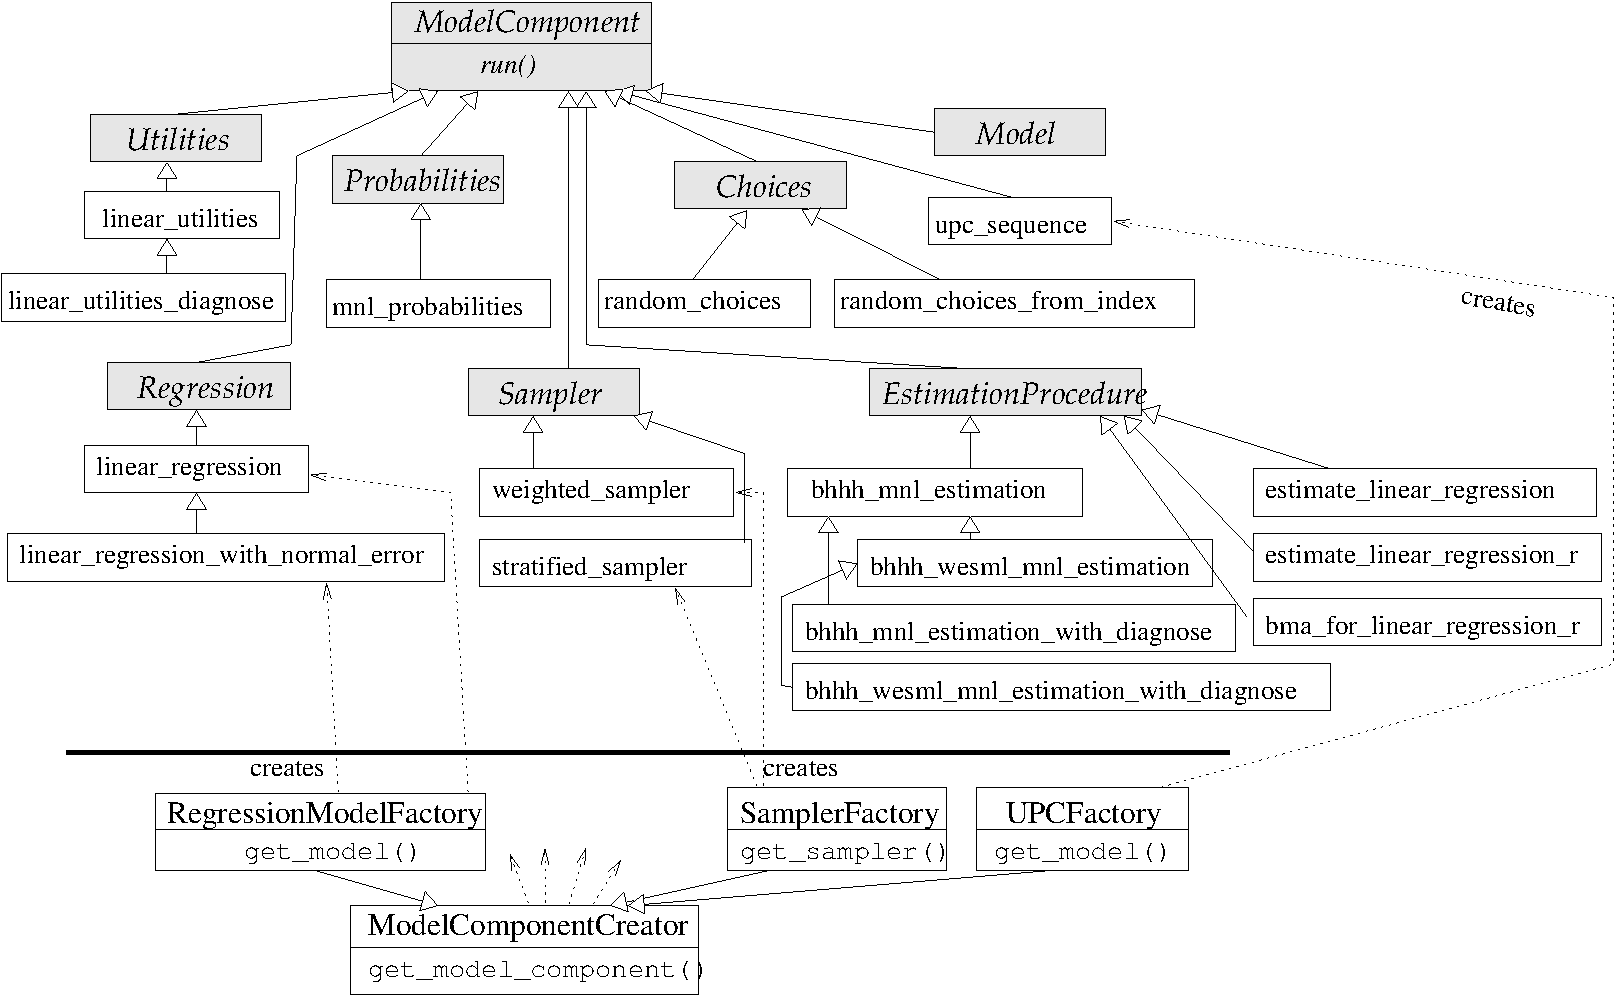
\includegraphics[scale=0.6]{images/corecomponents.pdf}
%end{latexonly}
\caption{\label{fig:model-components}\small Model components in Opus' \package{opus_core}.}
\htmlonly{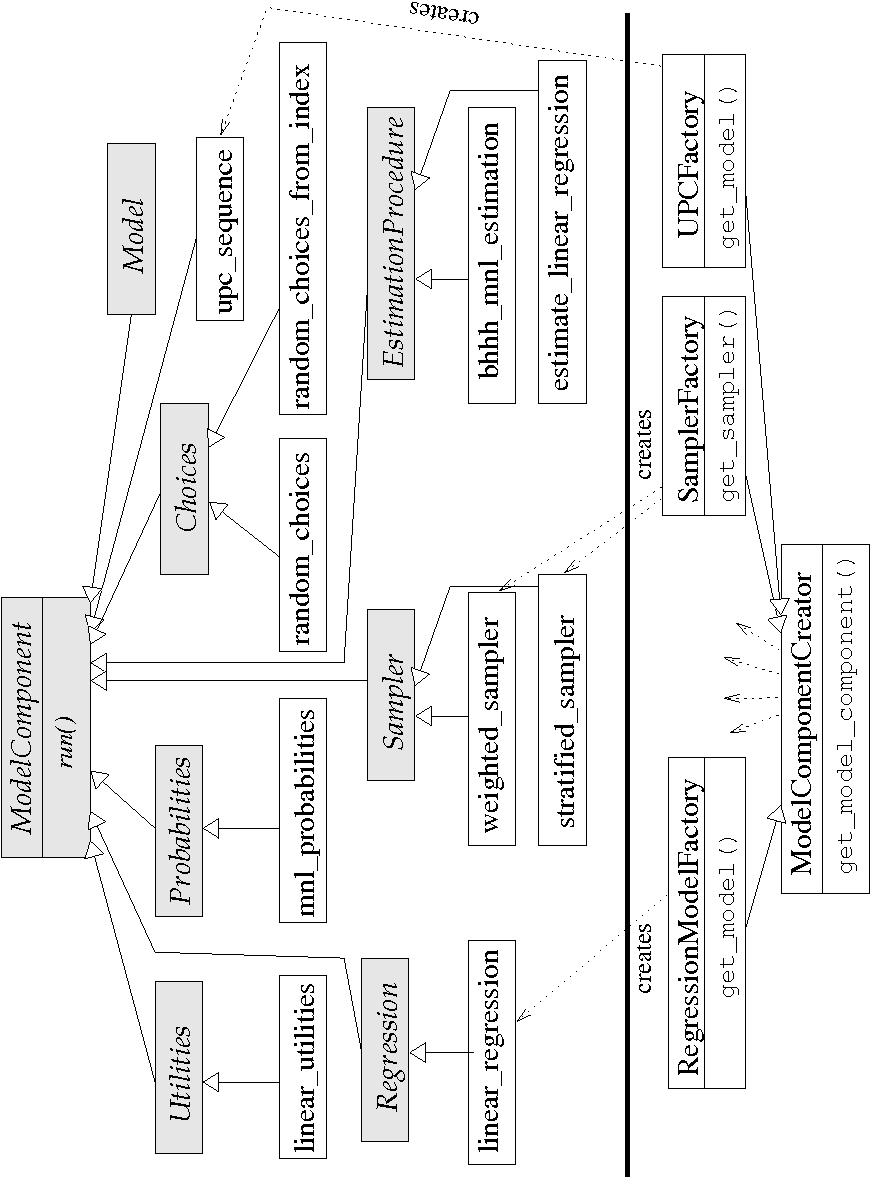
\includegraphics[scale=0.8]{images/corecomponents.jpg}}
\end{center}
\end{figure}

Instances of model components can be created using the class
\class{ModelComponentCreator}, by passing the class name into the method
\verb|get_model_component()|. In such a case the class name must be the same
as the module name. If it is not the case, one can use \class{ClassFactory}
for this purpose. There are a few child classes of
\class{ModelComponentCreator} implemented in \package{opus_core} for creating specific
model components.

\subsection{Utilities Class}
\label{sec:utilities}
\index{Utilities@\class{Utilities} class}
\index{utilities}
The \class{Utilities} class is used for computing utilities in
discrete choice modeling. In \package{opus_core} there is a
\class{Utilities} class implemented, called \class{linear_utilities}\index{linear_utilities@\class{linear_utilities}},
which computes linear utilities:
\[
U_{ni} = \sum_{j=1}^J \beta_{ij}x_{nij}\,.
\]
Here $i=1,\dots,I$ denotes the $I$ different alternatives, $n$ is an index for
observations (agents), $x$ denotes values of $J$ variables (including
constants) for each agent and alternative, and $\beta$ is a coefficient matrix
of size $I\times J$. The \verb|run()| method gets a 3-d array of data and a
2-d array of coefficients as arguments and returns a 2-d array of utilities.

A child class of \class{linear_utilities}, called
\class{linear_utilities_diagnose}\index{linear_utilities_diagnose@\class{linear_utilities_diagnose}}, 
serves analyzing changes in utilities 
due to changes in the data. For each variable set to its 5\%- and 95\%-quantile, respectively, while keeping
the remaining variables at their median, it runs the \class{linear_utilities} module. Results 
are stored in a file. First line of the file corresponds to the 5\%-quantile, second line to the 95\%-quantile,
and third line contains the difference between lines one and two. The name of the file 
can be passed to the \method{run()} method in its argument \verb|resources| as a dictionary key
'utilities_diagnose_file'. Default name is 'util'.



\subsection{Probabilities Class}
\label{sec:probabilities}
\index{Probabilities@\class{Probabilities} class} \index{probabilities}

The \class{Probabilities} class is an abstract class for computing
probabilities in the discrete choice modeling framework. Given
utilities $U$, the \package{opus_core} class {\bf
mnl_probabilities} \index{class!Probabilities!mnl_probabilities}\index{probabilities!MNL probabilities}
computes multinomial logit probabilities:
\[
P_{ni} = \frac{e^{U_{ni}}}{\sum_{j} e^{U_{nj}}}\,.
\]
Thus, the method \verb|run()| takes a 2-d array of utilities as an argument
(number of agents $\times$ number of alternatives) and returns a 2-d array of
probabilities (the same shape as utilities).

\subsection{Choices Class}
\label{sec:choices}
\index{Choices@\class{Choices} class}

\class{Choices} is an abstract class for selecting choices according to given
probabilities in the discrete choice modeling framework. Opus package \package{opus_core} supports
two classes in this category. {\bf random_choices} \index{class!Choices!random_choices} returns an index of
randomly selected choices, one per observation. The number of alternatives is
simply derived from the second dimension of the array of probabilities, which
is passed as argument to the \verb|run()| method. {\bf
  random_choices_from_index} \index{class!Choices!random_choices_from_index} allows one to define an index array whose
elements are returned as the selected choices. This index array should be
contained in the argument \verb|resources| (dictionary) as an entry \verb|index|. This can be
useful for example if we are not dealing with the whole set of alternatives,
but rather with a subsampled set.

\subsection{upc_sequence Class}
\label{sec:upc-sequence}
\index{class!upc_sequence}

In the discrete choice modeling framework, there is a certain order of steps
that need to be evaluated, namely computing utilities, computing
probabilities and selecting choices. This class allows to perform these steps
using just one method call.

The class \class{upc_sequence} is composed by an object of \class{Utilities},
an object of \class{Probabilities} and an object of \class{Choices}. The
objects are passed to the constructor. Alternatively, one can use the
\class{UPCFactory} class, which creates an \class{upc_sequence} object from
names (character strings) of the components.

The \method{run()} method calls the \method{run()} methods of the component
classes in the order given above, passing results from one class to the next
one as input values. Thus, the method takes a 3-d array of data and a 2-d
array of coefficients as arguments and returns an array of choices.  Any of
the components can be eliminated by setting it to None. In such a case, the
components receive results of the previously running component as input and
the results of the very last running method is the return value of the
\method{run()} method of \class{upc_sequence}.

\subsection{Regression Class}
\label{sec:regression}
\index{Regression@\class{Regression} class}\index{regression}

The \class{Regression} class is an abstract class for user defined classes
that can be used in the regression model. The class {\bf linear_regression} 
\index{class!Regression!linear_regression} \index{regression!linear regression}
implemented in \package{opus_core} computes outcome $Y$ as a linear combination of given
data $X$ and coefficients \boldmath $\beta$\unboldmath: $y_n = \sum_{j=1}^J
\beta_j x_{nj}$. Here, $J$ denotes the number of variables entering the
regression and $n$ is an index for observations. The \verb|run()| method takes
a 2-d array of data (of size number of observations $\times$ number of
variables) and a 1-d array of coefficients as arguments and returns a 1-d
array of outcome.

A child class of \class{linear_regression}, called {\bf linear_regression_with_normal_error}, 
\index{class!Regression!linear_regression_with_normal_error}
adds normaly distributed random errors to the outcome: $y_n = \sum_{j=1}^J \beta_j x_{nj} + \delta_n$ 
where $\delta_n \sim N(\mu_n, \sigma_n^2)$. $\mu_n$ and $\sigma_n^2$, respectively, can be passed 
to the \method{run()} method in its argument \verb|resources| (dictionary) as entries
'linear_regression_error_mean' and 'linear_regression_error_variance', respectively. Both can be specified either as 
a single value or as an array of size number of observations.
By default, $\delta_n \sim N(0, 1)$ for all $n$.


\subsection{EstimationProcedure Class}
\label{sec:estimation-procedure}
\index{EstimationProcedure@\class{EstimationProcedure} class}\index{estimation}
%
This class is an abstract class for modules that implement estimation of
coefficients for one of the available models. {\bf bhhh_mnl_estimation}
\index{class!EstimationProcedure!bhhh_mnl_estimation}\index{BHHH estimation}\index{estimation!BHHH estimation}
implements the BHHH estimation algorithm for multinomial logit models and can
be plugged into the \class{ChoiceModel}. As arguments, it gets a data array (of size number
of observations $\times$ number of alternatives $\times$ number of variables)
and an object \class{upc_sequence}. It uses the classes
\class{Probabilities} and \class{Utilities} contained in \class{upc_sequence}
for the maximum likelihood estimation. This assures that if
\class{bhhh_mnl_estimation} is plugged into the \method{estimate()} method of
\class{ChoiceModel} (Section~\ref{sec:choice-model}), the model will be
estimated by using the same code for computing utilities and probabilities as
the \verb|run()| method.  The third argument of the \verb|run()| method of
this class is of type \class{Resources} and must contain an entry
\verb|selected_choice| which is a 0-1 matrix of size number of observations
$\times$ number of alternatives. For each agent, it contains a 1 on a position
of the chosen alternative, otherwise 0s. Note that \class{ChoiceModel}
prepares and passes this matrix automatically.

A child class of \class{bhhh_mnl_estimation}, called {\bf bhhh_wesml_mnl_estimation}, 
\index{class!EstimationProcedure!bhhh_wesml_mnl_estimation}
implements 
the Weighted Endogenous Sampling Maximum Likelihood procedure, proposed by Manski, Lerman 1977.
Here, the data are weighted by correction weights (observation share/sampled share) in order to take into account 
undersampled or oversampled observations. The correction weights should be implemented
as a variable. Its fully-qualified name is passed to the \method{run()} method in the argument 
\verb|resources| (dictionary) as an entry 'wesml_sampling_correction_variable'.

Classes {\bf bhhh_mnl_estimation_with_diagnose} and {\bf bhhh_wesml_mnl_estimation_with_diagnose},
\index{class!EstimationProcedure!bhhh_mnl_estimation_with_diagnose}
\index{class!EstimationProcedure!bhhh_wesml_mnl_estimation_with_diagnose}
respectively, run the estimation of their parent classes, namely
\class{bhhh_mnl_estimation} and \class{bhhh_wesml_mnl_estimation}, respectively, using 
the utilities component \class{linear_utilities_diagnose} (see Section~\ref{sec:utilities}).

{\bf estimate_linear_regression} \index{class!EstimationProcedure!estimate_linear_regression}
performs a parameters estimation via the
least squares method. As arguments, it gets a data array (of size number of observations
$\times$ number of variables), an instance of class \class{Regression} (not
used in this module) and an object \class{Resources}. The last
argument must contain an entry \verb|outcome| which is a 1-d array of an outcome
for each observation. This class can be plugged into the
\class{RegressionModel} which takes care of all arguments.

{\bf estimate_linear_regression_r} \index{class!EstimationProcedure!estimate_linear_regression_r}
estimates the parameters using the R function lm. Here, the rpy module is required. It should 
give the same results as \class{estimate_linear_regression}.

The estimation modules return a dictionary with several entries: Entries \verb|estimators| and
\verb|standard_errors| contain arrays of estimated coefficients and their
standard errors, respectively. An entry \verb|other_measures| is a dictionary
which should contain additional measures of the estimates, i.e. their values
should be arrays of the same size as estimators. The two estimation modules
in \package{opus_core} return here one entry, namely the \verb|t_statistic|. The last entry in
the dictionary returned by the modules, \verb|other_info|, is a dictionary
containing additional information about the estimation. Its values don't
follow any restriction on type and size. Thus, these can be also single values,
such as likelihood ratio test statistics, degrees of freedom, $R^2$ etc.

Opus also implements a tool for variable selection in linear regression. Class 
{\bf bma_for_linear_regression_r} uses the R package BMA. 
It prints out results computed by the R function bic.glm and plots an image of the results.
The input arguments are identical to those in \class{estimate_linear_regression}. Additionally,
if the dictionary \verb|resources| contains an entry 'bma_imageplot_filename', the resulting imageplot 
is stored as a pdf file of that name. 
The \method{run()} method does not return any value. It should serve users as a tool to select variables 
which can be then plugged into \class{estimate_linear_regression}. The module rpy is required 
when using this component.

%% \subsection{sampling_toolbox}
%% \label{sec:samplingtoolbox} The sampling_toolbox is a collection of
%% sampling functions built upon numpy.  It provides equal
%% probability sampling with and without replacement
%% ({\it{sample_replace}} and {\it{sample_noreplace}} respectively),
%% unequal probability sampling with and without replacement ({\it{probsample_replace}}
%% and {\it{probsample_noreplace}} respectively), stratified sampling ({\it{stratifiedsample}}),
%% 2d sampling ({\it{prob2dsample}}), sampling (Monte Carlo(MC) or max_prob) ``choice'' from
%% a 2d probability array({\it{sample_choice}}), as well as functionality of normalization of
%% weight or probability ({\it{normalize}}) and finding duplicates ({\it{find_duplicates}} and
%% {\it{find_duplicates_others}}) in array.

%% Please refer to its source code sampling_toolbox.py in opus_core for detail usage.

\subsection{Sampler Class}
\label{sec:sampler}
\index{Sampler}
\index{Sampler@\class{Sampler} class}

The \class{Sampler} class is an abstract class for sampling alternatives for agents.
It returns 2-d array with rows representing agents and columns representing sampled
alternatives. It is not directly used in any \package{opus_core} model, but it is a building
block that can be used in models of other packages. For example, we made a
heavy use of this component in the \package{urbansim} package for creating sampled
alternative set for agents in \class{ChoiceModel}.

\subsubsection{Weighted Sampling}
\index{class!Sampler!weighted_sampling}
\index{weighted sampling}

{\bf weighted_sampling} is a child class of \class{Sampler} class.
It randomly samples alternatives from choice population with
probability proportion to their weights. Its \method{run()} method accepts the
following arguments:
\begin{description}
\item[dataset1] - an instance of \class{Dataset}, to be used as agent set.
\item[dataset2] - an instance of \class{Dataset}, to be used as choice set.
\item[index1] - indices of \verb|dataset1| for whom alternatives are sampled.
If it is not given, all elements of dataset1 are used.
\item[index2] - indices of \verb|dataset2| from which alternatives are
sampled. If it is not given, all elements of dataset2 are used.
\item[sample_size] - number of alternatives sampled.
\item[weight] - an array used as weight for elements of dataset2 in unequal
probability sampling; it has to be either of None, or of the same size as index2 or
dataset2. If it is not given, sampling is proceeded with equal probability.
\item[include_chosen_choice] - whether agents' chosen choice will be included in
the return results. If it's true, the chosen choices are in the first column of
the return results.
\item[resources] - an instance of \class{Resources} that can be used to pass any of
the above arguments to the run method.
\end{description}

\subsubsection{Stratified Sampling}
\index{class!Sampler!stratified_sampling}
\index{stratified sampling}

{\bf stratified_sampling} is a child class of \class{Sampler} class.
It randomly samples alternatives from choice population according to
their stratum setting. Its \method{run()} method accepts the following
arguments:
\begin{description}
\item[dataset1] - an instance of \class{Dataset}, to be used as agent set.
\item[dataset2] - an instance of \class{Dataset}, to be used as choice set.
\item[index1] - indices of \verb|dataset1| for whom alternatives are sampled.
If it is not given, all elements of dataset1 are used.
\item[index2] - indices of \verb|dataset2| from which alternatives are
sampled. If it is not given, all elements of dataset2 are used.
\item[stratum] - an array indicates the stratum id for elements of dataset2; it has
to be either of None, or of the same size as index2 or dataset2. If it's not given,
all elements are treated as in 1 stratum.
\item[weight] - like in weighted_sampling, weight is an array used as weight
for elements of dataset2 in unequal probability sampling; it has to be either
of None, or of the same size as index2 or dataset2. If it is not given, sampling
is proceeded with equal probability.
\item[sample_size] - number of alternatives sampled from one stratum; default value is 1.
\item[sample_size_from_chosen_stratum] - number of alternatives sampled from agent's chosen stratum.
If it's None, it's equal to value specified by sample_size or sample|_rate.
\item[sample_rate] - calculate number of alternatives sampled from one stratum by multiplying this rate with
number of observations in this stratum. If both sample_rate and sample_size are specified, use sample_rate.
\item[include_chosen_choice] - whether agents' chosen choice will be included in
the return results. If it's true, the chosen choices are in the first column of
the return results.
\item[resources] - an instance of \class{Resources} that can be used to pass any of
the above arguments to the run method.
\end{description}

Both sampling classes return a tuple where the first element is the sampled index, and the second element is 
the index within the sampled index indicating the chosen choice.

\section{Specification and Coefficients}
\label{sec:specification-coefficients}
%
\subsection{Specification}
\index{Specification}
\index{EquationSpecification@\class{EquationSpecification} class}\index{model!specification}
%
\label{sec:specification}
Often, models are specified by a set of variables. These are connected to a
set of coefficients calibrated to the observed data. Opus defines a class for
such specification, called \class{EquationSpecification}.

\subsubsection{Initialization}
The constructor of \class{EquationSpecification}
takes the following arguments (they all have default value None):
\begin{description}
\item[variables] - an array of variable names.
\item[coefficients] - an array  of coefficient names.
\item[equations] - an array of equations.
\item[submodels] - an array of submodels.
\item[fixed_values] - an array of fixed values. Any non-zero value is considered as a constant value
  of the corresponding coefficient, i.e. it is not to be estimated.
\item[other_fields] - a dictionary holding additional columns of the specification table.
\item[specification_dict] - the specification is specified in a dictionary format (see below). This argument 
 is considered only if the argument
  \verb|variables| is None. In such a case, all arguments above are ignored.
\item[in_storage] - an object of class \class{Storage} for loading
  specification from a storage.
\item[out_storage] - an object of class \class{Storage} for specification output.
\end{description}

All arguments are set as class properties.

The arrays \verb|variables| and \verb|coefficients| must have the same size.
If \verb|submodels|, \verb|equations| and \verb|fixed_values| are not omitted, they too must have
the same length as \verb|variables|. It is interpreted as the $i$-th variable
is connected to the $i$-th coefficient in the $i$-th equation (if there are
any) in the $i$-th submodel (if there are any). If the $i$-th fixed value is non-zero, the $i$-th coefficient
is not to be estimated. All entries of \verb|other_fields| must also be of the same size 
as \verb|variables|.
Values of \verb|equations| and
\verb|submodels| should be strictly positive integers. Coefficients should
have different names across equations, i.e. if there would be $i$ and $j$ for
which the \verb|coefficients[i]==coefficients[j]| and
\verb|equations[i]<>equations[j]| and \verb|submodels[i]==submodels[j]|, it
would lead to errors when connecting specification and coefficients.

An alternative way of defining a specification is a dictionary format (passed to the constructor via the argument 
\verb|specification_dict|).
Keys of the dictionary are submodels. If there
is only one submodel, the value $-2$ should be used as key. 
The value for each submodel entry is a list containing specification for the particular submodel.
The elements of each list can be defined in one of the following forms:
\begin{itemize}
\item a character string specifying a variable in its fully qualified name or as an expression. In such a case, 
      the coefficient name is determined by the alias of the variable.
\item a tuple of length 2: variable name as above, and the corresponding coefficient name.
\item a tuple of length 3: variable name, coefficient name, fixed value of the coefficient (if the 
                                coefficient should not be estimated).
\item a dictionary with pairs variable name, coefficient name
\end{itemize}
\verb|specification_dict| can contain an entry '_definition_' which should be a list of elements in one of the forms above.
In such a case, the entries defined for submodels can contain only the variable aliases. The corresponding 
coefficient names and fixed values (if defined) are taken from the definition section. Examples of specifications in 
a dictionary format can be found in the unit tests of the \class{EquationSpecification} class.


\subsubsection{Loading from and Writing into Storage}
%
If the specification is stored in one of the supported storage formats,
one can omit all arguments in the constructor and load the specification
from the storage, using the method \method{load()}. It takes the following
arguments:
\begin{description}
\item[resources] - an object of class \class{Resources}. If the remaining
  arguments are given, they will have priority over entries of the same name
  in \verb|resources|.
\item[in_storage] -  an object of class \class{Storage} that overwrites the
  one given in the constructor.
\item[in_table_name] - name of the table/file where the specification should
  be loaded from.
\item[variables] - if this argument is given, it serves as a filter for the
  variables loaded from the storage.
\end{description}
For each of the class properties variables, coefficients, equations,
submodels, and fixed_values, respectively, a table column is accepted on the storage (the first two are required, 
the others are optional). The column
names are given in the \verb|resources| entries 'field_variable_name',
'field_coefficient_name', 'field_equation_id', 'field_submodel_id', and 'field_fixed_value', 
respectively. Default values for the column names are \verb|'variable_name'|, 
 \verb|'coefficient_name'|,
\verb|'equation_id'|, \verb|'sub_model_id'|, and \verb|'fixed_value'|, respectively. If the table contains 
columns of other names, they are loaded into the class attribute other_fields, each as a dictionary entry. 

To store a specification into a storage, use the method
\method{write(resources, out_storage, out_table_name)}. The behavior is
analogous to the \method{load()} method. If equations or/and submodels are not
used, the method stores values $-2$ in those columns.


\subsection{Coefficients}

\label{sec:coefficients}
\index{Coefficients@\class{Coefficients} class}\index{model!coefficients}
%
Coefficients can be managed by the class \class{Coefficients}. Its behavior
is similar to the one of \class{EquationSpecification}.

\subsubsection{Initialization}
The constructor takes the following arguments:
\begin{description}
\item[names] - an array of coefficient names.
\item[values] - an array of coefficient values (of the same size as
  \verb|names| if not empty).
\item[standard_errors] - an array of standard errors of coefficients (of the
  same size as \verb|names| if not empty).
\item[submodels] - an array of submodels (of the same size as \verb|names| if
  not empty).
\item[in_storage] - an object of class \class{Storage} for loading
  coefficients from a storage.
\item[out_storage] - an object of class \class{Storage} for coefficients
  output.
\item[other_measures] - a dictionary for other coefficient measures, such as
  t-values. Keys are the names of the measures, values are arrays or of
  the same size as \verb|names|.
\item[other_info] - dictionary storing other information about the
  coefficients, such as goodness of fit values.
\end{description}
The arguments are interpreted as the coefficient of $i$-th name has the $i$-th
value, optionally the $i$-th standard error and is used in $i$-th
submodel. This also applies to each entry in \verb|other_measures|. Note that since
equations are not used here, there has to be coefficients with different names
for different equations, defined in the specification.

All arguments are set as class properties. 

%
\subsubsection{Loading from and Writing into Storage}
%
The method \method{load()} is similar to the one defined in
\class{EquationSpecification}. It takes the arguments:
\begin{description}
\item[resources] - an object of class \class{Resources}. If the remaining
  arguments are given, they will have priority over entries of the same name
  in \verb|resources|.
\item[in_storage] -  an object of class \class{Storage} that overwrites the
  one given in the constructor.
\item[in_table_name] - name of the table/file where the coefficients should
  be loaded from.
\end{description}
For each of the class properties names, values, standard errors, and
submodels, respectively, a table column is expected on the storage. 
The column names are given in the \verb|resources|
entries 'field_coefficient_name', 'field_estimate',
'field_standard_error', and 'field_submodel_id', respectively. Default
values for the column names are \verb|'variable_name'|, \verb|'coefficient_name'|, 
\verb|'equation_id'|, and \verb|'sub_model_id'|. If there are other fields in the table, their column names should be
given in the entry 'other_fields' of  \verb|resources| which is a list of character strings. The
default value is \verb|['t_statistic', 'p_value']|.

To store coefficients into a storage, use the method
\method{write(resources, out_storage, out_table_name)}. The behavior is
analogous to the \method{load()} method.

The class also allows to create a coefficient table in the \LaTeX
format. Method \method{make_tex_table()} accepts as arguments the file name
(without `.tex'), optionally the directory path and headers for each column.

\subsection{Specified Coefficients}
\label{sec:specified-coefficients}
\index{SpecifiedCoefficients@\class{SpecifiedCoefficients} class}
%
In order to connect a specification with coefficients, Opus uses the class
\class{SpecifiedCoefficients}. Its method \method{create()} takes an instance
of class \class{Coefficients} and an instance of class
\class{EquationSpecification} and creates arrays of coefficient values,
standard errors and other measures. The shape of those arrays is such that
they can be easily combined with data arrays when connecting coefficients to
variable values. In particular, they have three dimensions, number of
equations, number of variables and number of submodels.

For working with single submodels, there is a child class of
\class{SpecifiedCoefficients}, called
\class{SpecifiedCoefficientsFor1Submodel}, that is initialized by passing the
parent object and the submodel number.

Those classes are created and used by two \package{opus_core} models, namely regression model
for computing the regression and the choice model for computing the utilities.

\section{Other Classes}
%
\subsection{Dataset Pool}
\label{sec:core-dataset-pool}
\index{dataset pool}\index{DatasetPool@\class{DatasetPool} class}
%
A class called \class{DatasetPool} is designed to maintain a 'pool' of datasets. It is mainly used when
computing variables. Therefore in most cases, it will be only needed if the \class{Dataset} method
\method{compute_variables()} is used (for which an instance of \class{DatasetPool} is passed as an argument) in order
to have external datasets available that are required by the various variable implementations
 (see an example in Section~\ref{sec:variableconcept}).

The class is initialized by passing arguments:
\begin{description}
\item[package_order] - a list of packages that are used for finding the corresponding dataset class. Default is an empty list.
\item[package_order_exception] - a dictionary of exceptions from the \verb|package_order| as pairs dataset name
and list of packages for that dataset. Default is an empty dictionary.
\item[storage] - an object of class \class{Storage} that contains data of datasets to be included in pool. Default is \verb|None|.
\item[datasets_dict] - a dictionary containing pairs of dataset name and dataset object. Default is an empty dictionary.
\end{description}
One can add a dataset into the pool using the method \\
\method{_add_dataset(dataset_name, dataset)}, \\
or by
passing multiple datasets in one dictionary using the method \\
\method{add_datasets_if_not_included(datasets_dict)}.

A dataset can be accessed by the method \\
\method{get_dataset(dataset_name, dataset_arguments)}\\
 where the second argument is optional.
If a dataset of the given name is included in the pool, it is returned. Otherwise, the class creates a Dataset object using
the storage passed to the constructor. In order to create the appropriate Dataset class, it is searched
for a module called {\em dataset_name}\verb|_dataset.py| which should contain a class called {\em DatasetName}\verb|Dataset|.
The \class{DatasetPool} class searches for this module in the directory \file{datasets} of packages given in the initialization argument
'package_order'.

\subsection{ModelGroup and ModelGroupMember}
%
\label{sec:model-group}
\index{model group}\index{ModelGroup@\class{ModelGroup} class}
%
These two classes are designed to be used in models that are considered as model groups, i.e. models that are to be run
multiple times, each time on different subsets of one dataset.

A model group is defined by the following:
\begin{itemize}
\item There must be a dataset whose one attribute defines the names of the group members.
These names must be unique within the dataset.
We will call this dataset and its attribute {\em grouping dataset} and {\em grouping attribute} respectively.
Values of the unique identifier of the grouping dataset will be called  {\em member codes}.
\item A dataset that is going to be subset for running the model member on must contain an attribute whose values
represent the member codes. We will call this attribute {\em agents grouping attribute}.
\end{itemize}

Example: Suppose we would like to run a model on a 'job' dataset, subset according to its building type. Then
our grouping dataset, say 'job_building_type', can contain the following data:
\begin{verbatim}
id	name
1	'commercial'
2	'industrial'
3	'residential'
\end{verbatim}
The attribute 'name' is our grouping attribute, values of the 'id' attribute are member codes.
The dataset 'job' contains an attribute, say 'building_type' that has
value 1 for all commercial jobs, 2 for all industrial and 3 for all residential jobs. 'building_type' is then the
agents grouping attribute.

The class \class{ModelGroup} is initialized by
\begin{description}
\item[dataset] - object of class \class{Dataset} that is the grouping dataset.
\item[grouping_attribute] - name of the grouping attribute.
\end{description}
The class offers useful methods for accessing member names and codes of this group.

The class \class{ModelGroupMember}\index{ModelGroupMember@\class{ModelGroupMember} class}\index{model group member} is initialized by
\begin{description}
\item[model_group] - object of class \class{ModelGroup}.
\item[member_name] - name of this specific member. It must be contained in the grouping attribute of 'model_group'.
\end{description}
A model that uses this class should use the method \method{set_agents_grouping_attribute(attribute)} to set
the agents grouping attribute. Then the class can be used for subsetting any dataset according to the member codes,
e.g. by the method \method{get_index_of_my_agents(dataset, index)} which selects those entries from the given index that
correspond to this group member.

\subsection{Configuration Classes}
\label{sec:resources} 
%
Opus implements a few classes that are used for configuration of objects.
\begin{description}
\item[\class{GeneralResources}] -- \index{GeneralResources@\class{GeneralResources} class} a Python dictionary with some additional methods.
\item[\class{SessionConfiguration}] -- \index{SessionConfiguration@\class{SessionConfiguration} class} a singleton class
        (subclass of \class{GeneralResources}) that is to be configured
        with global settings for a user's session.  Requires parameter
        \verb|in_storage| to not be \verb|None| if creating a new instance, so
        SessionConfiguration knows from where to get the data for any dataset it
        creates.
\item[\class{Configuration}] -- \index{Configuration@\class{Configuration} class} 
  a child of \class{GeneralResources} that implements a hierarchical
        representation of the user-specified parameters and settings.
\item[\class{Resources}] -- \index{Resources@\class{Resources} class} a child of \class{Configuration}. It has access to the
\class{SessionConfiguration}.
\item[\class{ChunkSpecification}] -- \index{ChunkSpecification@\class{ChunkSpecification} class} class for configuring chunks used by the \class{ChunkModel} (see 
Section~\ref{sec:chunk-model}). It is initialized by a dictionary containing either the key `records_per_chunk' or
`nchunks' with the appropriate value. Method \method{nchunks()} returns number of chunks. Method \method{chunk_size()}
returns the number of records in one chunk.
\end{description}

%%% Local Variables:
%%% mode: latex
%%% TeX-master: "userguide"
%%% End:

% LocalWords:  tex borning uninstall Dataset SimulationState AttributeCache Un
% LocalWords:  MySQL versioning gridcell un VariableName AttributeBox rpy ij ln
% LocalWords:  matplotlib DatasetSubset indices InteractionDataset attr
% LocalWords:  ChoiceModel attrtype valuetypes mysql Bool
% LocalWords:  StorageFactory columnwise txt urbansim DDD powDDD gridcells faz
% LocalWords:  numpy py VariableFactory UInt pre ds ChunkModel chunked upc
% LocalWords:  RegressionModel ChunkSpecification submodel submodels config ni
% LocalWords:  EquationSpecification RegressionModelFactory ClassFactory nij nj
% LocalWords:  ModelComponentCreator mnl logit subsampled UPCFactory bhhh bla
% LocalWords:  EstimationProcedure UrbanSim SpecifiedCoefficients userguide
% LocalWords:  SpecifiedCoefficientsFor
